\section{Introduction}
Accurate depth estimation remains a central problem in robotic perception, underpinning tasks such as navigation, mapping, and interaction.
As discussed in Chapter~\ref{ch:intro}, recent advances have explored a spectrum of approaches, ranging from classical geometric optimization and self-supervised learning from monocular video to emerging feed-forward geometry Transformers.
Despite these developments, stereo matching continues to play a uniquely important role due to its ability to provide metrically grounded depth through explicit geometric constraints.

However, stereo matching itself presents a long-standing challenge: the need to resolve ambiguous correspondences in the presence of textureless regions, repetitive patterns, occlusions, and reflective surfaces.
Traditional methods address this problem through carefully designed regularization schemes, often formulated as Markov Random Fields (MRFs), where spatial smoothness and discontinuity-preserving priors are explicitly encoded and optimized.
While these approaches offer strong geometric interpretability, they typically rely on hand-crafted potentials and computationally expensive inference procedures.
In contrast, modern learning-based stereo methods achieve remarkable performance by leveraging deep neural networks to learn matching costs and regularization implicitly.
Yet, this implicit formulation often sacrifices interpretability and struggles to robustly enforce global consistency, particularly in challenging regions where local evidence is weak or ambiguous. 
This tension between explicit structured reasoning and learned representations motivates the approach presented in this chapter. 
We revisit the classical MRF formulation for stereo matching and propose to bridge it with modern deep learning.
Specifically, we introduce a \emph{Neural Markov Random Field (NMRF)}, in which both the unary and pairwise potentials are parameterized by neural networks, while the structured inference framework that enforces global consistency is preserved.

By integrating learnable representations with principled probabilistic modeling, the proposed NMRF combines the strengths of classical and deep stereo methods: it retains the structured reasoning of MRF-based approaches while benefiting from the expressive power of neural networks.
This design enables robust disparity estimation in challenging scenarios, including occluded regions and complex geometric boundaries.
More broadly, this work reflects a recurring theme of this thesis: the integration of geometric structure with learned representations.
While later chapters explore learning unified geometric representations, the NMRF framework acts as an earlier but important step in this direction, emphasizing structured reasoning over learned features within the stereo matching problem.

The remainder of this chapter is organized as follows.

\section{Neural MRF Formulation}\label{sec:mrf-model}
Given a rectified stereo image pair, consisting of a left image $I^L$ and a right image $I^R$, binocular stereo matching aims to estimate a dense disparity map $D: \Omega \mapsto \mathbb{R}^+$, where where $\Omega \subset \mathbb{Z}^2$ denotes the pixel coordinate domain.
For a pixel $\mathbf{p} = (i,j)$ in the left image, its corresponding point in the right image appears at $\mathbf{p}' = (i, j-d)$ under the rectified epipolar geometry, where $d > 0$ is the disparity.
The depth is then recovered as $f \cdot b / d$, with $f$ the focal length and $b$ the baseline distance.

We formulate stereo matching as a discrete labeling problem, where each pixel $o$ in $I_L$ is assigned a candidate disparity draw from a finite set $L_o \subset \mathbb{R}^+$.
Classical MRF-based approaches minimize an energy function over assignments $\{z_o \mid z_o \in L_o\}$ and rely on pairwise smoothness terms to regularize the solution.
However, such formulations typically model interactions using simple functions of disparity differences (\eg, $|z_o - z_p|$), which limits their ability to capture richer contextual and geometric relationships~\cite{szeliski2008comparative}.
To address this limitation, we propose a Neural Markov Random Field (NMRF).
In our framework, each candidate label is associated with an embedding vector $\mathbf{z}_v \in \mathbb{R}^d$. 
This representation enables the model to encode not only disparity values but also higher-level geometric and contextual information.

Formally, we construct a graph $\mathcal{G} = (\mathcal{V}, \mathcal{E})$ over all candidate labels, where each node $v \in \mathcal{V}$ corresponds to a pixel–disparity pair.
The joint distribution over observed features $\{\mathbf{x}_v\}$ and latent embeddings $\{\mathbf{z}_v\}$ is defined as
\begin{equation}
	p(\{\mathbf{x}_v\}, \{\mathbf{z}_v\}) \propto \prod_{v \in \mathcal{V}} \Phi(\mathbf{x}_v, \mathbf{z}_v)\prod_{(u,v)\in \mathcal{E}} \Psi(\mathbf{z}_u, \mathbf{z}_v),
\end{equation}
where $\Phi(\mathbf{x}_v, \mathbf{z}_v)$ denotes a unary potential relating the observed feature $\mathbf{x}_v$ to its latent representation, and $\Psi(\mathbf{z}_u, \mathbf{z}_v)$ encodes pairwise compatibility between neighboring labels.

The graph structure incorporates two distinct types of interactions.
First, \emph{intra-pixel} (self) edges connect all candidate labels belonging to the same pixel, enforcing competition among alternative disparity hypotheses.
Second, \emph{inter-pixel} (neighbor) edges connect labels across spatially adjacent pixels within a local $M \times M$ window, encouraging spatial consistency.
Unlike conventional stereo MRFs that often neglect intra-pixel interactions, we explicitly model both types using separate potential functions, $\Psi_{\tt{self}}$ and $\Psi_{\mathrm{neigh}}$, respectively.
Intuitively, $\Psi_{\mathrm{neigh}}$ promotes agreement between compatible disparities across neighboring pixels, while $\Psi_{\mathrm{self}}$ suppresses conflicting assignments at the same pixel. This distinction introduces a useful inductive bias that improves solution quality.
In contrast to traditional MRF formulations where $\Phi$ and $\Psi$ are manually designed, the proposed NMRF learns these interactions implicitly through the latent embeddings $\{\mathbf{z}_v\}$. The learning objective drives the embeddings to be consistent with the ground truth disparity map.

\section{Neural MRF Inference}\label{sec:mrf-inference}
\subsection{Embedding Mean-Field Inference}
Exact inference of the posterior $p(\{\mathbf{z}_v\} \mid \{\mathbf{x}_v\})$ is computationally intractable due to the densely connected structure of the graph.
To enable efficient inference, we adopt a mean-field approximation, in which the joint posterior is factorized into a product of independent marginal distributions:
\begin{equation}
	p(\{\mathbf{z}_v\} \mid \{\mathbf{x}_v\}) \approx \prod_{v} q_v(\mathbf{z}_v \mid \mathbf{x}_v).
\end{equation}
The optimal set of marginals $\{q_v\}$ are obtained by minimizing the Kullback–Leibler (KL) divergence between the approximate and true posteriors~\cite{dai2016discriminative}.

Under this approximation, each marginal distribution must satisfy a fixed-point condition~\cite{hamilton2020graph}:
\begin{equation}
	\log q_v(\mathbf{z}_v) = c_v + \log \Phi(\mathbf{x}_v, \mathbf{z}_v) + \sum_{u \in \mathcal{N}(v)} \int_{\mathbb{R}^d} q_u(\mathbf{z}_u)\log \Psi(\mathbf{z}_u, \mathbf{z}_v) \mathrm{d}\mathbf{z}_u,
	\label{eq:fixed-point}
\end{equation}
where $c_v$ is a normalization constant and $\mathcal{N}(v)$ denotes the set of neighboring nodes of $v$.
This equation highlights that the marginal at each node depends not only on the local observation $\mathbf{x}_v$ but also on the distributions of its neighbors.
To obtain a tractable implementation, we represent each marginal distribution using a finite-dimensional embedding.
Assuming the existence of an injective feature map $\phi(\cdot)$, we define
\begin{equation}
	\mu_v = \int_{\mathbb{R}^d} q_v(\mathbf{z}_v)\phi(\mathbf{z}_v)\mathrm{d}\mathbf{z}_v \in \mathbb{R}^d,
\end{equation}
which serves as a compact representation of $q_v$.
The fixed-point updates can then be approximated in the embedding space through an iterative message passing procedure:
\begin{equation}
	\mu_v^{t} = \tilde{f}\big(\mathbf{x}_v, \mu_v^{t-1}, \{\mu_u^{t-1}\}_{u \in \mathcal{N}(v)}\big),
	\label{eq:em-update}
\end{equation}
where $\tilde{f}$ is a vector-valued message passing function that encapsulates the complex, nonlinear dependencies induced by the potential functions $\Phi$, $\Psi$, and the feature map $\phi$.
This formulation naturally leads to a message passing mechanism, in which inference is implemented as iterative refinement of node embeddings.

\subsection{Inference with Neural Message Passing}
Mean-field inference is analytically tractable only for restricted classes of potential functions, such as those belonging to the exponential family.
In our setting, however, the potential functions $\Phi$, $\Psi$, as well as the feature map $\phi$, are not specified a priori and must be learned from data.
As a result, the exact functional form of the update operator $\tilde{f}$ in Equation~\ref{eq:em-update} is unknown and cannot be derived in closed form.
To address this, we parameterize $\tilde{f}$ using a neural network designed to emulate the structure of mean-field updates.
Specifically, the network performs iterative message passing over the graph, where each node updates its embedding by aggregating information from its neighbors and combining the result with its current embedding.
This procedure can be interpreted as a learned approximation to the fixed-point iteration arising from the mean-field formulation.

We initialize the embedding of each node $v$ with its observed feature, \ie, $^{(0)}\mu_v = \mathbf{x}_v$.
Let $^{(\ell)}\mu_v$ denote the embedding at iteration (or layer) $\ell$.
The update from layer $\ell$ to $\ell+1$ consists of two steps: \emph{message aggregation} and \emph{feature transformation}.
Denoting by $\mathbf{m}_{\mathcal{E}^\ell \rightarrow v}$ the aggregated message from the edge set $\mathcal{E}^\ell \in \{\mathcal{E}_{\mathrm{self}}, \mathcal{E}_{\mathrm{neigh}}\}$ into node $v$, the update rule is defined as
\begin{equation}
	\begin{aligned}
		^{(\ell+1)}\hat{\mu}_v &= ^{(\ell)}\mu_v + \mathbf{m}_{\mathcal{E}^\ell \rightarrow v}\\
		^{(\ell+1)}\mu_v &= \mathrm{MLP}\left(^{(\ell+1)}\hat{\mu}_v\right) + ^{(\ell+1)}\hat{\mu}_v,
	\end{aligned}
	\label{eq:msg-passing}
\end{equation}
where the residual connection facilitates stable iterative refinement.
This formulation admits a natural interpretation in the context of mean-field inference. The aggregation term $\mathbf{m}_{\mathcal{E}^\ell \rightarrow v}$ corresponds to the influence of neighboring marginals, analogous to the pairwise interaction term $\Psi(\cdot,\cdot)$ in Equation~\ref{eq:fixed-point}. The subsequent transformation via the MLP plays a role similar to the unary potential $\Phi$, modulating the embedding based on local evidence.
Each layer sequentially aggregates information along the \emph{self} and \emph{neighbor} edges before updating the embedding.
By stacking $N_i$ such layers, the network performs iterative refinement of the embeddings, progressively approximating the mean-field inference.

\subsection{Attentional Message Aggregation}
To model pairwise interactions, we implement the message aggregation operator using an attention mechanism, which naturally captures \emph{affinity} between nodes.
For aggregation along inter-pixel edges $\mathcal{E}_{\mathrm{neigh}}$, each node $v$ aggregates information from its neighboring nodes $\{u : (u,v) \in \mathcal{E}_{\mathrm{neigh}}\}$ through a weighted combination:
\begin{equation}
	\begin{aligned}
		\mathbf{m}_{\mathcal{E}_{\mathrm{neigh}} \rightarrow v}
		&= \sum_{(u,v)\in\mathcal{E}_{\mathrm{neigh}}} \alpha_{uv} \big(\mathbf{v}_u + \mathbf{r}^{\mathrm{v}}_{u-v}\big)\\
		\alpha_{uv}
		&= \mathrm{softmax}_u \Big( \mathbf{q}_v^\top \mathbf{k}_u
		+ \mathbf{q}_v^\top \mathbf{r}^{\mathrm{k}}_{u-v}
		+ \mathbf{k}_u^\top \mathbf{r}^{\mathrm{q}}_{u-v} \Big),
	\end{aligned}
	\label{eq:nmrf_agg}
\end{equation}
where $\mathbf{q}_v$, $\mathbf{k}_u$, and $\mathbf{v}_u$ denote the query, key, and value vectors obtained via linear projections of the node embeddings. The terms $\mathbf{r}^{\mathrm{q}}_{u-v}$, $\mathbf{r}^{\mathrm{k}}_{u-v}$, and $\mathbf{r}^{\mathrm{v}}_{u-v}$ encode the relative position $\mathbf{p}_u-\mathbf{p}_v$ between nodes $u$ and $v$ in three different subspaces.
This attention-based formulation can be interpreted as a learned instantiation of the pairwise potential $\Psi$, where the attention weights $\alpha_{uv}$ quantify the compatibility between candidate labels.
Incorporating relative positional encodings $\mathbf{r}_{u-v}^\mathrm{v}$ in aggregation enables the model to capture both spatial and disparity relationships, which is particularly beneficial in ambiguous regions where geometric context is critical.
Meanwhile, the query $\mathbf{q}_v$ and key $\mathbf{k}_u$ encode content-dependent cues that guide where each node attends within its neighborhood.
Their interactions with the relative positional encodings introduce a \emph{content-adaptive positional bias}, allowing spatial relationships to be modulated according to local appearance. 
This mechanism is particularly important for stereo matching, where ambiguities arising from textureless or repetitive patterns can be mitigated by incorporating geometric priors. Similar forms of positional bias have also been shown to be effective in prior work such as STTR~\cite{li2021revisiting}.

Concretely, the relative position $\mathbf{p}_u - \mathbf{p}_v$ is defined in a 3D space comprising pixel offsets $(\Delta i, \Delta j)$ and disparity difference $\Delta d$. 
Directly encoding this quantity for all label pairs is computationally prohibitive due to its quadratic complexity. 
Instead, we adopt an efficient approximation. 
The spatial offsets $(\Delta i, \Delta j)$, constrained within a local $M \times M$ window, are encoded using a learnable lookup table $\mathbf{P} \in \mathbb{R}^{3 \times (2M-1) \times (2M-1) \times D}$, where the leading dimension corresponds to the query, key, and value embeddings, respectively. 
For the disparity component, we encode the absolute disparity using a sinusoidal representation, which is concatenated with the node embedding prior to linear projections.
For intra-pixel edges $\mathcal{E}_{\mathrm{self}}$, all nodes correspond to the same spatial location, and thus the spatial offsets vanish. 
In this case, the relative positional encoding terms related to $(\Delta i, \Delta j)$ are omitted, resulting in a simplified aggregation that focuses on competition among disparity candidates.

\section{Network Architecture}

\begin{figure}[!t]
	\centering
	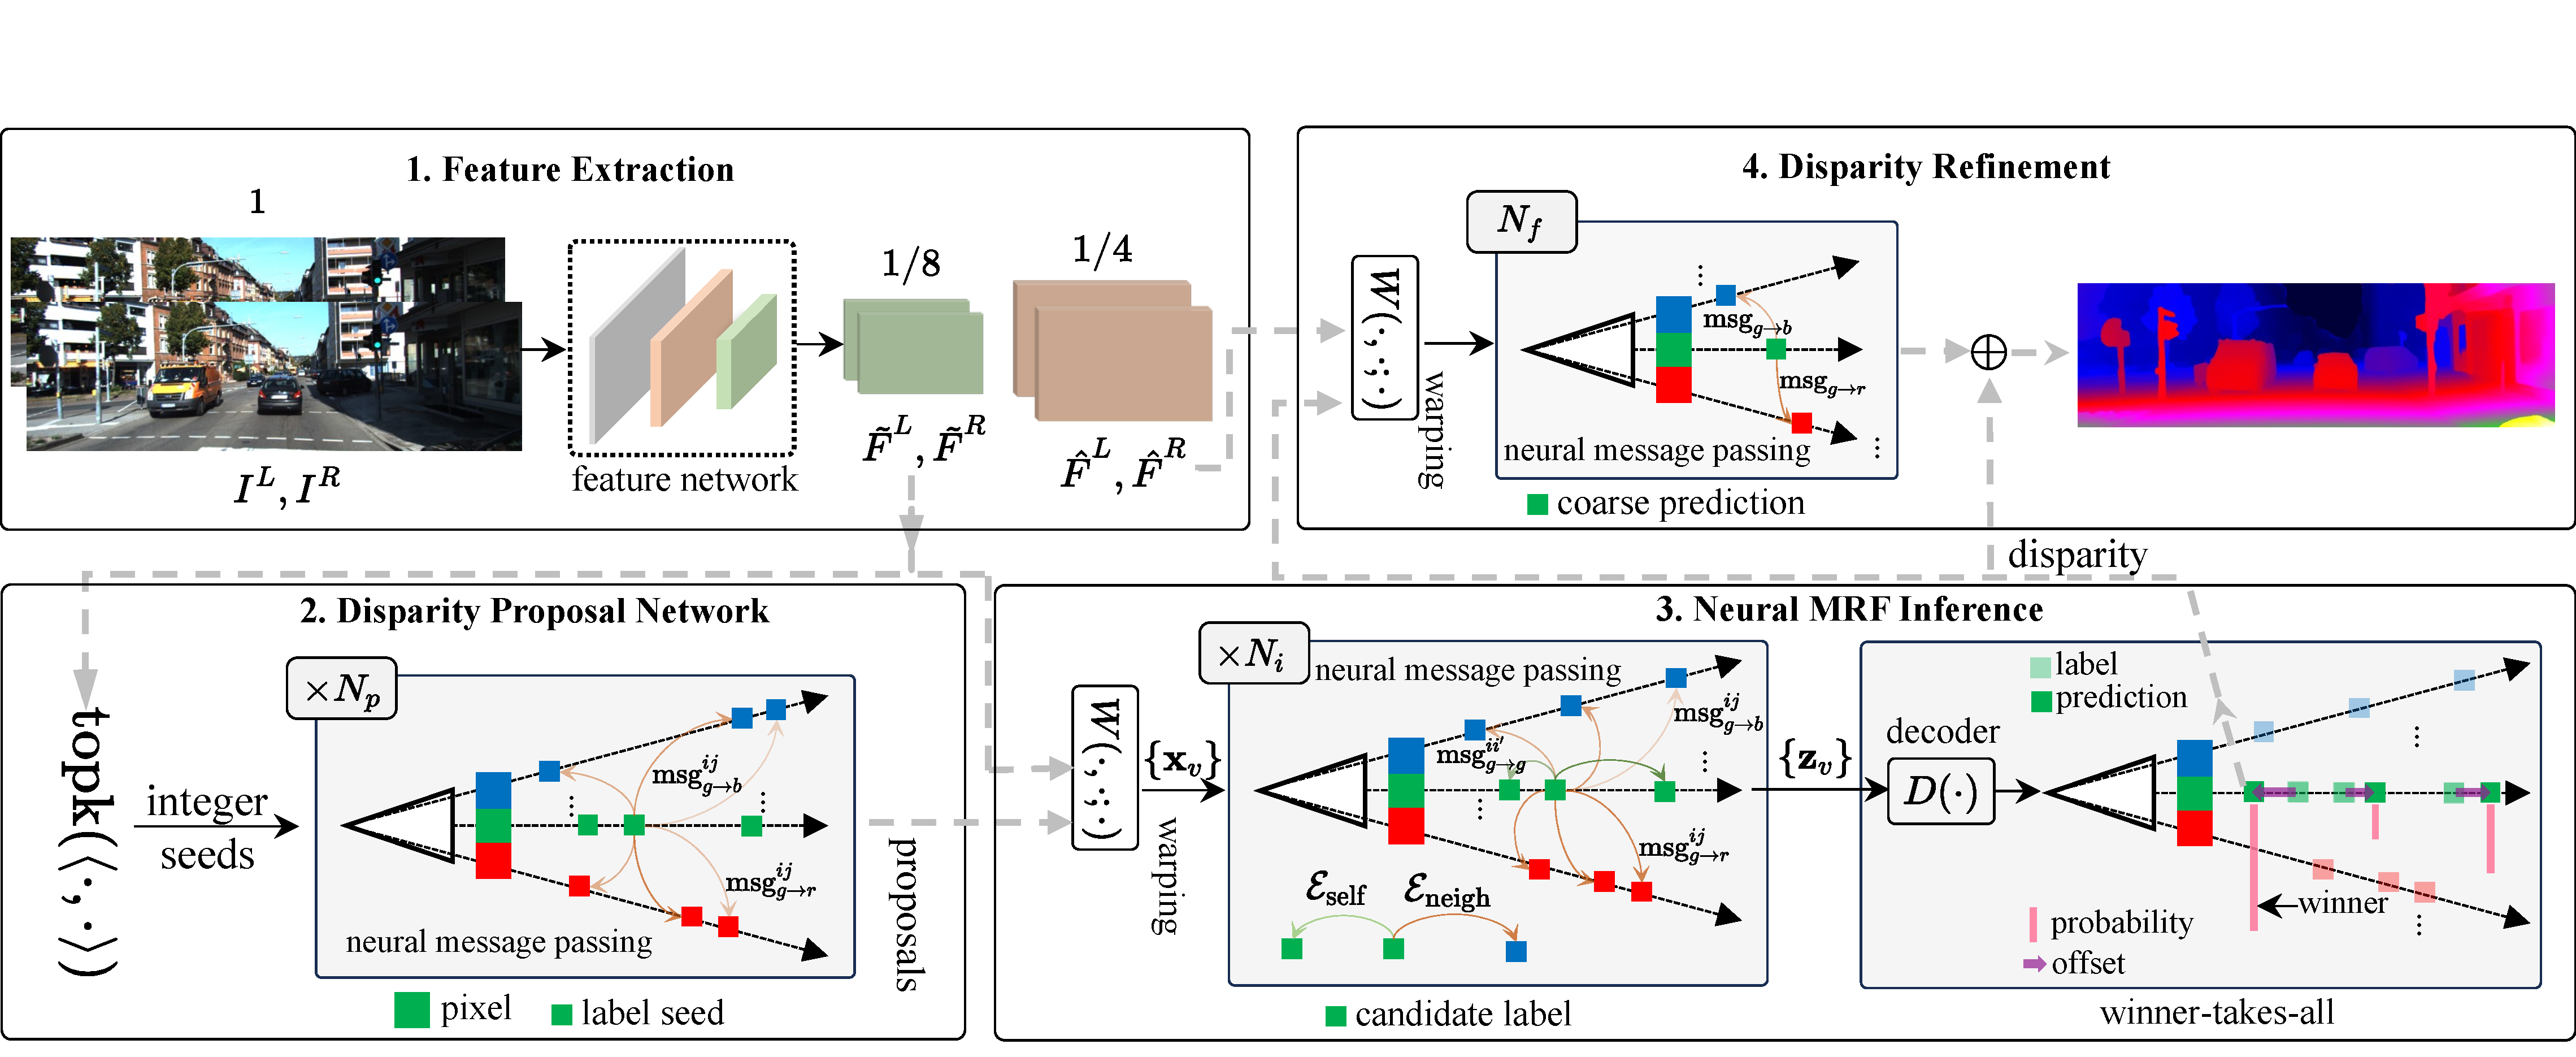
\includegraphics[width=0.99\linewidth]{fig/nmrf/overview.pdf}
	\vspace{-0.3em}
	\caption{\textbf{Architecture of the proposed NMRF model.} The pipeline consists of four submodules. \textbf{1.} A feature extraction network processes the input stereo pair and produces both coarse- and fine-level feature maps. 
		\textbf{2.} A disparity proposal network prunes the search space by selecting the top-$k$ candidate disparity modals for each pixel, which are further refined through $N_p$ iterations of neural message passing, yielding $k$ candidate disparity labels per pixel.
		\textbf{3.} These candidates are organized into a probabilistic graph, where each node represents a candidate label and edges connect labels across neighboring pixels. Distinct potential functions are employed for intra- and inter-pixel interactions. The latent embeddings $\{\mathbf{z}_v\}$  for each pixel are then decoded into posterior probabilities and offsets, from which the most likely label is selected as the coarse disparity estimate.
		\textbf{4.} A subsequent refinement applies a lightweight neural MRF with a single label per pixel, where the inferred embeddings are used to predict residual corrections for the final disparity.}
		\label{fig:nmrf_overview}
		\vspace{-0.2em}
\end{figure}
This section presents the implementation of the Neural Markov Random Field (NMRF) framework introduced in Sections~\ref{sec:mrf-model} and~\ref{sec:mrf-inference}.
An overview of the full architecture is shown in Figure~\ref{fig:nmrf_overview}.
This model follows a  two-stage design. 
In the first stage, an NMRF is applied at a coarse spatial resolution ($\nicefrac{1}{8}$ of the input image size) to produce an initial disparity estimate (Section~\ref{sec:nmrf_inference_network}).
To ensure computational tractability, we introduce a Disparity Proposal Network that significantly prunes the search space (Section~\ref{sec:dpn}).
In the second stage, the coarse predictions is refined at a higher resolution ($\nicefrac{1}{4}$ of the input size) features using a lightweight NMRF. 
Both stages are supported by a shared feature extraction network that provides both coarse- and fine-level features.

\subsection{Feature Extraction}\label{sec:nmrf_backbone}
Given a rectified stereo pair $(I^L, I^R)$, we employ a Siamese feature extractor to compute hierarchical feature representations.
Specifically, coarse-level features at $\nicefrac{1}{8}$ resolution are denoted as $\tilde{F}^L$ and $\tilde{F}^R$, while fine-level features at $\nicefrac{1}{4}$ resolution are denoted as $\hat{F}^L$ and $\hat{F}^R$.
These features play a critical role in stereo matching, especially in addressing challenges posed by occlusions, textureless regions, and varying lighting conditions.
However, achieving more expressive feature representations typically entails increased computation overhead.
To address the latency requirements of diverse applications, two feature network variants are introduced to balance performance and efficiency.

\begin{figure}[!t]
	\centering
	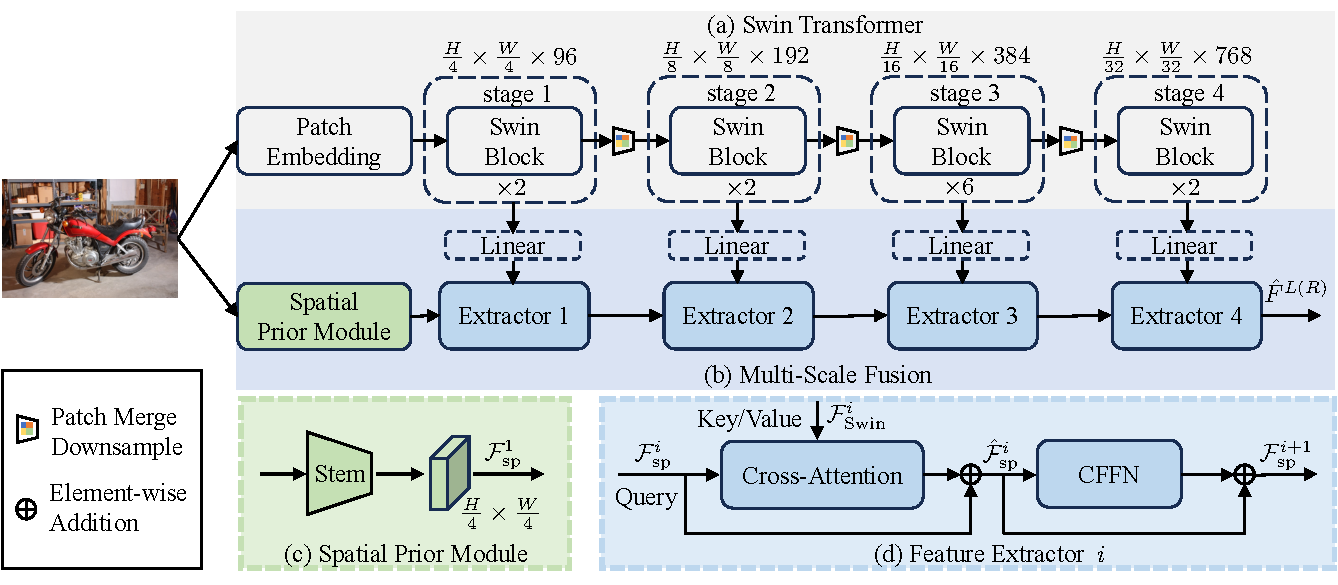
\includegraphics[width=0.99\linewidth]{fig/nmrf/backbone.pdf}
	\vspace{-0.3em}
	\caption{\textbf{Architecture of the performant feature network.} (a) The Swin-Tiny backbone, which produces hierarchical multi-scale features. (b) The multi-scale feature fusion strategy, which incorporates two key designs, including (c) a spatial prior module that captures local spatial contexts from the input image, and (d) a feature extractor that combines multi-scale features using the resolution-independent deformable attention~\cite{zhu2020deformable}.}
	\label{fig:nmrf_backbone}
	\vspace{-1.2em}
\end{figure}

\noindent\textbf{ResNet feature network.} For efficiency-critical settings, we adopt a lightweight convolutional backbone.
The input images $I^{L(R)} \in \mathbb{R}^{3 \times H \times W}$ are first downsampled to half resolution using a $7 \times 7$ convolution.
Feature extraction is then performed using a sequence of six residual blocks: two blocks at $\nicefrac{1}{2}$ resolution with 64 channels, followed by two blocks at $\nicefrac{1}{4}$ resolution with 96 channels, and two additional blocks at $\nicefrac{1}{4}$ resolution with 128 channels.
A final $1 \times 1$ convolution projects the features to obtain the fine-level representations $\hat{F}^L, \hat{F}^R \in \mathbb{R}^{256 \times \frac{H}{4} \times \frac{W}{4}}$.
The coarse-level features $\tilde{F}^L$ and $\tilde{F}^R$ are subsequently obtained by applying stride-2 average pooling to the fine-level features.
Instance normalization is used throughout the network to improve generalization performance~\cite{lipson2021raft}.

\noindent\textbf{Vision Transformer backbone}
To prioritize accuracy, we further explore feature extraction based on pre-trained vision transformers. Prior work~\cite{zhang2024exploring} has shown that transformer-based backbones, such as Swin~\cite{liu2021Swin} and Twins~\cite{chu2021twins}, provide stronger representations for stereo matching by leveraging rich instance-level semantics.
Motivated by this, we adopt an ImageNet-pretrained Swin-Tiny backbone and enhance it with a multi-scale feature fusion mechanism based on deformable attention, following ViT-Adaptor~\cite{chen2022vision} and Deformable Neck~\cite{zhang2024exploring}.
As illustrated in Figure~\ref{fig:nmrf_backbone}, the Swin backbone produces hierarchical features at multiple resolutions, which are progressively fused into a unified representation.

To strengthen local spatial modeling, we incorporate the Spatial Prior Module from ViT-Adaptor~\cite{chen2022vision}, which generates an initial feature map $\mathcal{F}_{\mathrm{sp}}^1$ containing fine-grained structural information.
This feature serves as the query in a sequence of deformable cross-attention layers.
At each stage, the spatial features are updated by attending to the corresponding Swin features:
\begin{align}
	\hat{\mathcal{F}}_{\mathrm{sp}}^i &= \mathcal{F}_{\mathrm{sp}}^i + \mathrm{Attention}\big(\mathrm{norm}(\mathcal{F}_{\mathrm{sp}}^i), \mathrm{norm}(\mathcal{F}_{\mathrm{Swin}}^i)\big)\\
	\mathcal{F}_{\mathrm{sp}}^{i+1} &= \hat{\mathcal{F}}_{\mathrm{sp}}^i + \mathrm{CFFN}\big(\mathrm{norm}(\hat{\mathcal{F}}_{\mathrm{sp}}^i)\big),
\end{align}
where $\mathcal{F}_{\mathrm{sp}}^i$ acts as the query, and $\mathcal{F}_{\mathrm{Swin}}^i$ provides the key and value. 
The convolutional feed-forward network (CFFN) uses a reduced expansion ratio of 0.25 to limit computational overhead.
The outputs from multi-scale fusion are used as the fine-level representations $\hat{F}^L, \hat{F}^R \in \mathbb{R}^{128 \times \frac{H}{4} \times \frac{W}{4}}$, while coarse-level features $\tilde{F}^L, \tilde{F}^R$ are obtained via average pooling.

\subsection{Disparity Proposal Network}\label{sec:dpn}
Direct inference over the full disparity space is computationally prohibitive for the proposed NMRF inference (Section~\ref{sec:mrf-inference}) due to the large number of candidate labels per pixel. 
To make inference tractable, we introduce a Disparity Proposal Network (DPN) that adaptively reduces the search space by selecting a compact set of reliable disparity candidates for each pixel. 
The DPN first identifies a sparse collection of promising disparity hypotheses and subsequently refines them through neural message passing, yielding $K$ high-quality disparity proposals per pixel.

\noindent\textbf{Top-$K$  Label Seeds.}
For a pixel $o=(i,j)$, the initial matching score for an integer disparity $d \in [0, d_{\mathrm{max}}]$ is computed via feature correlation:
\begin{equation}
	\mathbf{C}(i,j,d)=\langle \tilde{F}^L(i,j), \tilde{F}^R(i,j-d)\rangle.
\end{equation}
Rather than densely evaluating all disparity candidates during subsequent inference, we first identify a sparse set of representative disparity modals. 
Specifically, local maxima along the disparity dimension are detected using one-dimensional max pooling with kernel size $3$, corresponding to a local neighborhood of $[-1,1]$. 
A \verb|topk| operation is then applied to select the $k$ most confident modals.
Each selected modal is represented as a \emph{label seed} $(\mathbf{p}, \mathbf{d})$, consisting of a 3D position $\mathbf{p}$ and an associated matching descriptor $\mathbf{d}$. The position is defined as
\begin{equation}
	\mathbf{p}_v := (i,j,d),
\end{equation}
which encodes the pixel coordinates together with the candidate disparity. 
The matching descriptor is designed to capture both local matching evidence and disparity-aware geometric cues:
\begin{equation}
	\mathbf{d}_v=
	\mathrm{Linear}
	\Big(
	\delta_1\big(L_d(\mathbf{C}(i,j,:))\big)
	\, || \,
	\mathrm{PE}(d)
	\Big),
\end{equation}
where $L_d$ extracts local cost features centered at disparity $d$, following the strategy of RAFT-Stereo~\cite{lipson2021raft}. 
The extracted features are first normalized through a two-layer feed-forward network $\delta_1$, and subsequently concatenated with the sinusoidal positional encoding of disparity $d$. 
A linear projection is then applied to fuse appearance and geometric information into a unified representation.

\begin{figure}[!t]
	\centering
	\begin{subfigure}[t]{0.25\linewidth}
		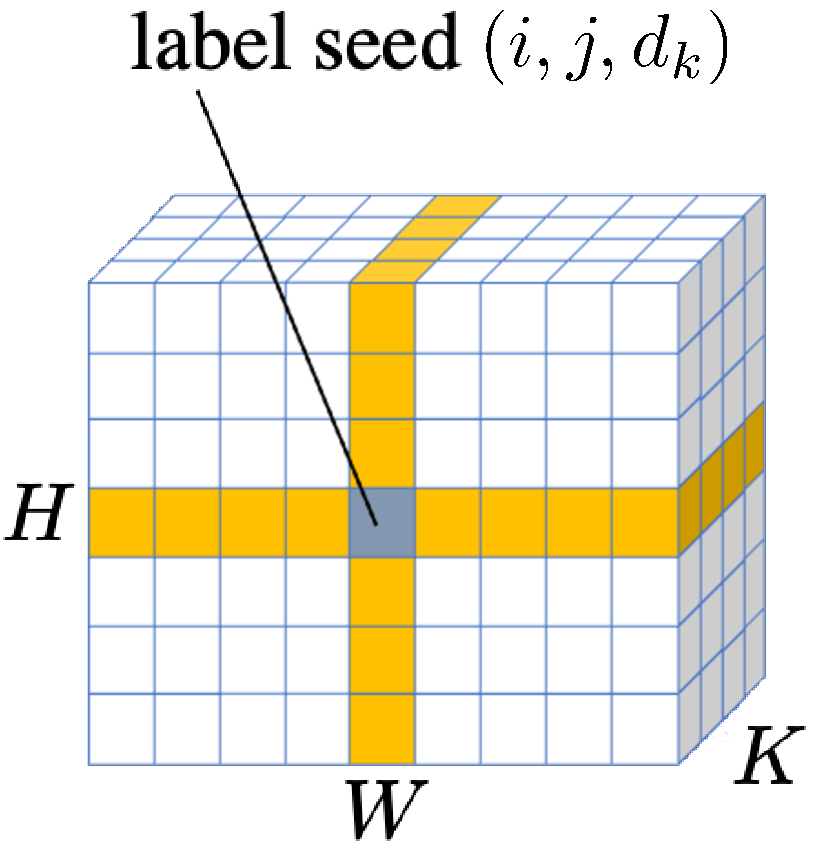
\includegraphics[width=\linewidth]{fig/nmrf/cross-shaped.pdf}
		\caption{}
		\label{fig:cross-shaped}
	\end{subfigure}
	\begin{subfigure}[t]{0.25\linewidth}
		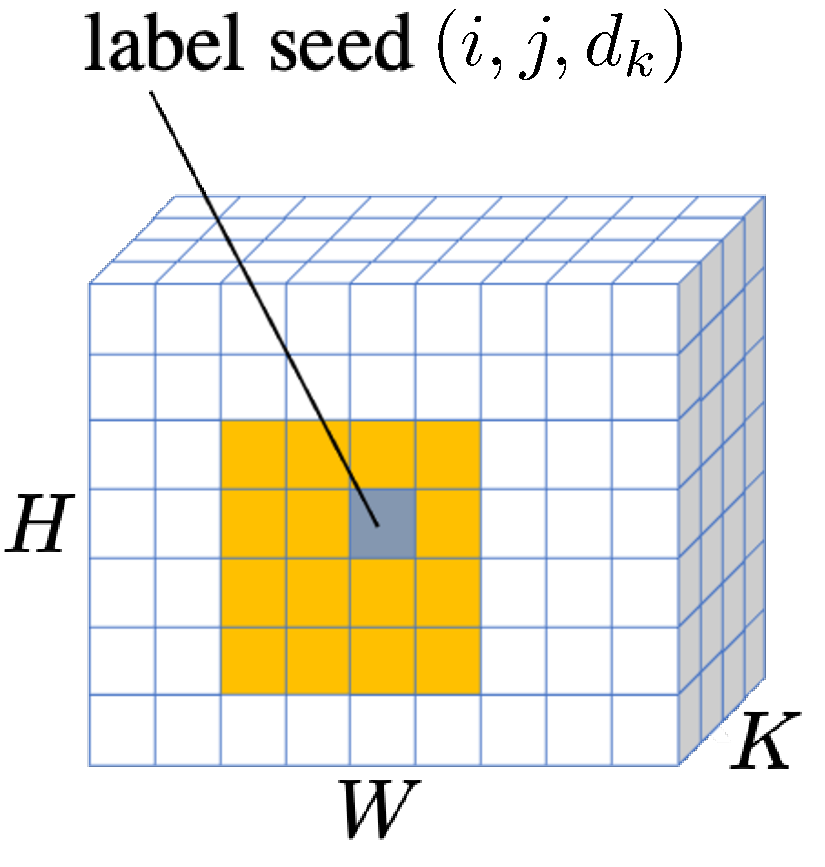
\includegraphics[width=\linewidth]{fig/nmrf/local-window.pdf}
		\caption{}
		\label{fig:local-win}
	\end{subfigure}
	\vspace{-1.0em}
	\caption{(a) Cross-shaped attention window layout, (b) local attention window layout.}  
	\vspace{-1.2em}
\end{figure}

\noindent\textbf{Label seed propagation.}
Although the top-$k$ label seeds provide strong initial hypotheses, they may still fail in challenging regions such as occlusions, reflective surfaces, or weakly textured areas. 
Nevertheless, correctly estimated seeds remain dominant across most parts of the image. 
This observation motivates the use of message passing to propagate reliable disparity cues toward ambiguous regions. 
Specifically, the neural message passing operation defined in Equation~\ref{eq:msg-passing} enables each label seed to incorporate contextual information from neighboring reliable hypotheses, thereby correcting erroneous or unstable disparity proposals.
Long-range interactions are particularly important for resolving large textureless regions and occluded areas. 
To efficiently capture such dependencies, we adopt the cross-shaped window self-attention mechanism of CSWin Transformer~\cite{dong2022cswin}. 
As shown in Figure~\ref{fig:cross-shaped}, a label seed located at $\mathbf{p}_v=(i,j,d)$ aggregates information from other seeds sharing either the same row index $i$ or column index $j$. 
This design enables efficient communication over large spatial extents while maintaining manageable computational complexity.
The propagation follows the \emph{parallel multi-head grouping} strategy and \emph{locally enhanced positional encoding} proposed in CSWin Transformer~\cite{dong2022cswin}.
In contrast to NMRF inference network (Section~\ref{sec:nmrf_inference_network}), the DPN excludes intra-pixel (\emph{self}) edges, since competition among candidate disparities is not required during proposal generation.
After $N_p$ iterations of message passing, the refined seed descriptors are decoded by a three-layer feed-forward network to predict residual corrections with respect to the initial integer disparity hypotheses.

To examine the effectiveness of the proposed cross-shaped attention design, we compare it with a conventional local window attention scheme illustrated in Figure~\ref{fig:local-win}.
For a fair comparison, the local attention window is configured to $8 \times 8$, resulting in a computational cost comparable to that of the cross-shaped attention on the SceneFlow dataset~\cite{mayer2016large} (\ie, $540\times 960$ resolution).
The quantitative comparison is presented in Table~\ref{tab:proposal_attention}.
The results indicate that cross-shaped attention yields more accurate disparity proposals, which can be attributed to its stronger capability for modeling long-range spatial dependencies during label seed propagation.

\subsection{Neural MRF Inference Network}\label{sec:nmrf_inference_network}
As illustrated in Figure~\ref{fig:nmrf_overview}(3), the NMRF inference network estimates the latent embeddings $\{\mathbf{z}_v\}$ from the observed label features $\{\mathbf{x}_v\}$ through $N_i$ iterations of neural message passing.
The resulting embeddings are subsequently decoded to produce disparity predictions.
While the general formulation of neural message passing has been introduced in Section~\ref{sec:mrf-inference}, this section describes the remaining components required for practical stereo inference.

\noindent\textbf{Observed Label Features.}
For each candidate label $v$ in the MRF graph, the observed feature $\mathbf{x}_v$ should jointly encode matching evidence from both stereo views.
Given the coarse-level feature maps $\tilde{F}^L$ and $\tilde{F}^R$, we construct the observed feature for a candidate located at $\mathbf{p}_v := (i,j,\hat{d})$ using a feature warping operation between $\tilde{F}^L(i,j)$ and $\tilde{F}^R(i,j-\hat{d})$:
\begin{align}
	\mathbf{x}_v
	&=
	\mathrm{MLP}
	\left(
	\mathbf{x}_v^{\mathrm{concat}}
	\, || \,
	\mathbf{x}_v^{\mathrm{corr}}
	\right), \nonumber \\
	\mathbf{x}_v^{\mathrm{concat}}(i,j,\hat{d})
	&=
	\delta_2\big(\tilde{F}^L(i,j)\big)
	\, || \,
	\delta_2\big(\tilde{F}^R(i,j-\hat{d})\big), \\
	\mathbf{x}_{v,g}^{\mathrm{corr}}(i,j,\hat{d},g)
	&=
	\frac{N_g}{N_c}
	\left\langle
	\delta_3\big(\tilde{F}_g^L(i,j)\big),
	\delta_3\big(\tilde{F}_g^R(i,j-\hat{d})\big)
	\right\rangle. \nonumber
\end{align}
Here, $\tilde{F}_g^L$ and $\tilde{F}_g^R$ denote the $g$-th feature groups obtained by evenly partitioning the coarse-level features into $N_g$ groups, while $N_c$ represents the total number of feature channels.
The term $\mathbf{x}_v^{\mathrm{concat}}$ captures appearance information through feature concatenation, whereas $\mathbf{x}_v^{\mathrm{corr}}$ measures matching similarity via grouped correlations.
The normalization functions $\delta_2$ and $\delta_3$ are introduced to align the feature distributions of the two components before fusion.
Both functions are implemented using a $3 \times 3$ convolution followed by instance normalization and ReLU activation, together with a subsequent $1 \times 1$ convolution layer.
Since the candidate disparity $\hat{d}$ may take continuous values after proposal refinement, bilinear interpolation is used when sampling the right-view feature map $\tilde{F}^R$.

\noindent\textbf{Disparity estimation.}
After $N_i$ iterations of neural message passing, the refined latent embeddings $\{^{(N_i)}\mu_v\}$ are decoded into disparity predictions.
For each coarse-level pixel, the embedding associated with every candidate label is processed independently to predict both disparity offsets and their corresponding confidence scores.
Specifically, a three-layer feed-forward network with ReLU activations regresses an $8 \times 8$ grid of disparity offsets relative to the candidate label. 
In parallel, a linear projection followed by a softmax operation estimates the posterior probability of each candidate. 
The predicted offsets are added to their associated candidate disparities, producing dense disparity hypotheses at the original image resolution.
Consequently, each input pixel $(i,j)$ is associated with a set of $K$ disparity hypotheses $\mathcal{H}_{ij}$, together with their estimated probabilities. 
The final disparity value is obtained using a winner-takes-all selection strategy, as illustrated in Figure~\ref{fig:nmrf_overview}(3).

\subsection{Disparity Refinement}\label{sec:nmrf_refinement}
The coarse-level NMRF inference already achieves strong performance, as demonstrated in Table~\ref{tab:ablation_comp}.
Nevertheless, fine-scale structures and object boundaries can be further improved through an additional refinement stage operating on higher-resolution features.
To this end, we perform $N_f$ iterations of neural message passing on the fine-level feature representations to refine the disparity estimation.
For computational efficiency, the refinement stage maintains only a single candidate label for each pixel.
The initial label is obtained by downsampling the coarse disparity prediction using stride-4 median pooling with a $4 \times 4$ kernel, producing a robust initialization at the fine feature resolution.
The resulting refinement graph differs from the coarse inference stage in two important aspects.
First, since each pixel contains only one disparity hypothesis, intra-pixel is no longer necessary, and therefore the graph contains no \emph{self} edges.
Second, the posterior probability prediction branch used during coarse inference is removed, as candidate selection is no longer required.
Consequently, the refinement stage focuses solely on propagating contextual information and predicting residual disparity corrections for enhanced structural detail.

\section{Loss Functions}
Our stereo network is trained end-to-end with losses applied to different stages of the pipeline, including label initialization, proposal extraction, multi-label MRF inference, and single-label disparity refinement.
These losses supervise complementary aspects of the model: the initialization loss encourages the cost volume to preserve plausible disparity modals, the proposal loss ensures that the extracted candidate labels cover the ground-truth disparity distribution within the local $8\times 8$ window, the multi-label disparity loss guides probabilistic MRF inference toward accurate hypotheses, and the refinement loss improves the final disparity accuracy.
Let $\Omega$ denote the set of valid pixels.
The overall training objective is defined as
\begin{equation}
	L_{\textsf{total}}
	=
	\lambda_{\textsf{init}} L^{\textsf{init}}
	+
	\lambda_{\textsf{prop}} L^{\textsf{prop}}
	+
	\lambda_{\textsf{disp}} L^{\textsf{disp}}
	+
	\lambda_{\textsf{ref}} L^{\textsf{ref}},
	\label{eq:total_loss}
\end{equation}
where $\lambda_{\textsf{init}}$, $\lambda_{\textsf{prop}}$, $\lambda_{\textsf{disp}}$, and $\lambda_{\textsf{ref}}$ balance the contributions of the four terms.
In our experiments, these weights are set empirically and kept fixed for all datasets unless otherwise specified.

\subsection{Initialization Loss}
The DPN first extracts label seeds from a 3D matching cost volume.
The purpose of the initialization loss is to encourage this cost volume to assign high responses to disparity modals that are likely to explain the local ground truth patch.
At the coarse resolution, each pixel $o$ corresponds to an image patch $\Omega_o$ in the original image.
Since $\Omega_o$ may contain multiple disparity modals, especially near object boundaries or thin structures, we construct a multi-modal target distribution from the valid disparities inside the patch.
Each valid disparity is first scaled to the coarse resolution by a factor of $8$, and then softly scattered to its two neighboring integer disparity bins using linear interpolation.
The scattered contributions from all valid pixels in $\Omega_o$  are accumulated and normalized into a probability distribution $\tilde{p}_o^*(d)$. 
Let $p_o(d)$ be the predicted disparity probability obtained by applying softmax to cost volume along the disparity dimension. 
The initialization loss is defined as the cross entropy between the patch-level soft target distribution and the predicted probability:
\begin{equation}
	L^{\textsf{init}}
	=
	-
	\frac{1}{|\Omega_{\textsf{init}}|}
	\sum_{o\in\Omega_{\textsf{init}}}
	\sum_{d=0}^{d_{\max}}
	\tilde{p}_o^*(d)
	\log p_o(d),
	\label{eq:init-loss}
\end{equation}
where $\Omega_{\textsf{init}}$ denotes the set of coarse-level pixels whose corresponding patch contains at least one valid ground truth disparity.
This soft cross-entropy loss encourages the initial cost volume to preserve the dominant disparity modals inside each local patch while still allowing secondary structures, boundary regions, and thin objects to contribute to seed selection.

\subsection{Proposal Loss}
While the initialization loss supervises the cost volume before seed selection, the proposal loss directly constraints the candidate labels after proposal extraction.
Let $L_o=\{\hat{d}_{o,k}\}_{k=1}^{K}$ be the set of candidate disparities proposed for coarse-level pixel $o$.
Ideally, these candidates should cover the ground-truth disparity values within the corresponding image patch $\Omega_o$.
For each valid pixel $p\in\Omega_o$, we identify the closest candidate label as
\begin{equation}
	\hat{\sigma}(p)
	=
	\arg\min_{k}
	\left| d_p^*-\hat{d}_{o,k} \right|.
	\label{eq:nearest-proposal}
\end{equation} 
The proposal loss is defined by minimizing the distance between each ground truth disparity and its nearest candidate:
\begin{equation}
	L^{\textsf{prop}}
	=
	\sum_o
	\sum_{p\in\Omega_o}
	\rho
	\left(
	d_p^*-\hat{d}_{o,\hat{\sigma}(p)}
	\right),
	\label{eq:l-prop}
\end{equation}
where $\rho(\cdot)$ denotes the Smooth-$L_1$ penalty.
This objective encourages the proposal network to generate a compact yet expressive set of candidate labels that can represent both smooth regions and locally multi-modal disparity structures.

\subsection{Multi-Label Disparity Loss}
After proposal extraction, neural MRF inference estimates a posterior distribution over the candidate disparity hypotheses. 
For pixel $(i,j)$, let $\mathcal{H}_{ij}$ denote the hypothesis set and let $p_{ij}(d')$ be the inferred posterior probability of hypothesis $d'\in\mathcal{H}_{ij}$. 
The multi-label disparity loss minimizes the expected absolute disparity error under this posterior distribution:
\begin{equation}
	L^{\textsf{disp}}
	=
	\sum_{(i,j)\in\Omega}
	\sum_{d'\in\mathcal{H}_{ij}}
	p_{ij}(d')
	\left| d'-d_{ij}^* \right|.
	\label{eq:loss-est}
\end{equation}
This loss favors posterior distributions whose probability mass is concentrated around accurate disparity hypotheses. 
Compared with supervising only the most likely label, the expectation-based formulation provides gradients to all hypotheses and therefore encourages both better probability estimation and more effective hypothesis refinement during neural message passing. 

\subsection{Refinement Loss}

The final refinement module predicts a continuous full-resolution disparity map $d$ from the output of coarse-level neural MRF inference. 
This stage is supervised using a direct regression loss between the refined disparity prediction and the ground-truth disparity map:
\begin{equation}
	L^{\textsf{ref}}
	=
	\sum_{(i,j)\in\Omega}
	\left|
	z_{ij}-z_{ij}^* 
	\right|.
	\label{eq:l-ref}
\end{equation}
This loss encourages the refinement module to recover fine-grained disparity details and sharpen local structures that may be smoothed in coarse-level multi-label inference.

\section{Experiments}
This section evaluates the proposed NMRF stereo framework from three perspectives: benchmark accuracy, cross-domain generalization, and component-level effectiveness.
To accommodate different computational requirements, two model variants are considered.
The efficiency-oriented variant, denoted as \emph{NMRF-light}, adopts the lightweight ResNet backbone introduced in Section~\ref{sec:nmrf_backbone} and maintains two candidate disparity labels for each pixel.
The accuracy-oriented variant denoted as \emph{NMRF-SwinT}, use the Swin Transformer~\cite{liu2021Swin} backbone described in Section~\ref{sec:nmrf_backbone} and retains four candidate labels per pixel.

Experiments are conducted on SceneFlow~\cite{mayer2016large}, KITTI~\cite{geiger2012we,menze2015object}.
SceneFlow is a large-scale synthetic stereo dataset containing 35,454 training pairs and 4,370 testing pairs with image resolution $540\times 960$ and dense ground-truth disparities.
KITTI 2012~\cite{geiger2012we} and KITTI 2015~\cite{menze2015object} are real-world autonomous driving benchmarks whose training sets provide sparse LiDAR-based disparity annotations.
KITTI 2012 contains 194 training pairs and 195 testing pairs, while KITTI 2015 contains 200 training pairs and 200 testing pairs.
For zero-shot evaluation, models trained only on SceneFlow are directly tested on the training splits of KITTI, Middlebury 2014~\cite{scharstein2014high}, and ETH3D~\cite{schops2017multi}.

\begin{table}[!t]
	\small
	\centering
	\caption{\textbf{Quantitative evaluation on SceneFlow test set.} Our NMRF-SwinT outperforms state-of-the-arts on both metrics.}
	\vspace{-0.6em}
	\resizebox{\linewidth}{!}{
	\begin{tabular}{c c c c c c c c c}
		\toprule 
		\textbf{Methods} & GANet~\cite{Zhang2019GANet} &  AANet~\cite{xu2020aanet} & 
		LEAStereo~\cite{cheng2020hierarchical} & ACVNet~\cite{xu2022attention} & IGEV-Stereo~\cite{xu2023iterative} & NMRF-light & NMRF-SwinT\\
		\midrule
		\textbf{EPE} [px] $\downarrow$ & 0.78 & 0.87 & 0.78 & 0.48 & 0.47 & 0.46 & \textbf{0.36}\\
		\textbf{Bad 1.0} [\%] $\downarrow$ &8.7&9.3&7.82&5.02&5.35&4.51&\textbf{3.64}\\
		\bottomrule
	\end{tabular}
	}
	\label{tab:results_sceneflow}
\end{table}

\subsection{Implementation Details}
All models are implemented in PyTorch and trained on NVIDIA RTX 3090 GPUs.
We use the AdamW optimizer together with a one-cycle learning-rate schedule for all training stages.
On SceneFlow, models are trained for 300k iterations with a batch size of 8.
Input images are randomly cropped to $384\times 768$, and the maximum learning rate is set to $5\times10^{-4}$.
Following the common SceneFlow evaluation protocol, pixels with ground-truth disparities larger than 192 are excluded during testing.
For KITTI benchmark submission, the SceneFlow pretrained model is further fine-tuned on the combined training images of KITTI 2012 and KITTI 2015.
Fine-tuning is performed for 39k iterations with a batch size of 4, using random crops of size $304\times 1152$ and a maximum learning rate of $2\times10^{-4}$.
Standard data augmentations are applied, including color jittering, eraser augmentation, and spatial transformation~\cite{lipson2021raft}.
Unless otherwise stated, all variants follow the same optimization and augmentation settings to ensure fair comparison.

\subsection{Benchmark Evaluation}

\begin{table}[!t]
	\small
	\centering
	\caption{\textbf{Evaluation on KITTI 2012 and 2015.} On KITTI 2012, we report the bad-$x$ error, \ie, the percentage of pixels with disparity error larger than $x$ pixels, for both non-occluded regions (noc) and all regions (all), together with the EPE on non-occluded pixels. On KITTI 2015, we report the D1 error for background (BG), foreground (FG), and all pixels. The best result is shown in \textbf{bold}, and the second-best result is \underline{underlined}.}
	\vspace{-0.3em}
	\resizebox{\linewidth}{!}{
	\begin{tabular}{c c c c c c c c c c}
		\toprule
		& \multicolumn{5}{c}{KITTI 2012} & \multicolumn{3}{c}{KITTI 2015} &\\
		\cmidrule(lr){2-6}
		\cmidrule(lr){7-9}
		\textbf{Methods} & \multicolumn{2}{c}{\textbf{bad 2.0}} & \multicolumn{2}{c}{\textbf{bad 3.0}} & \textbf{EPE}  
		& \textbf{BG} & \textbf{FG} & \textbf{ALL} & \textbf{Runtime}\\
		\cmidrule(lr){2-3}
		\cmidrule(lr){4-5}
		& noc [\%] &  all [\%] &  noc [\%] &  all [\%] & noc [px] & \multicolumn{3}{c}{All Areas [\%]} & [s] \\
		\cmidrule(lr){1-6}
		\cmidrule(lr){7-10}
		GCNet~\cite{kendall2017end} & 2.71 & 3.46  & 1.77 & 2.30 & 0.6 &  2.21 & 6.16 &  2.87 & 0.9\\
		PSMNet~\cite{chang2018pyramid} & 2.44 & 3.01 & 1.49 & 1.89  & 0.5 & 1.86 & 4.62 &  2.32 & 0.41\\  
		GwcNet~\cite{guo2019group} & 2.16 & 2.71 & 1.32 & 1.70 & 0.5 & 1.74 & 3.93 & 2.11 & 0.32\\
		GANet-deep~\cite{Zhang2019GANet}  & 1.89 & 2.50 & 1.19 & 1.60 &\textbf{0.4}      &1.48 &3.46 & 1.81 & 1.8 \\
		CSPN~\cite{cheng2019learning} & 1.79 & 2.27 & 1.19 & 1.53 & - & 1.51 & \underline{2.88} & 1.74 & 1.0\\
		RAFT-Stereo~\cite{lipson2021raft} & 1.92 & 2.42 & 1.30 & 1.66 & \textbf{0.4} & 1.58 & 3.05 & 1.82 & 0.38\\
		LEAStereo~\cite{cheng2020hierarchical} & 1.90 & 2.39 & 1.13 & 1.45 & 0.5 & 1.40 & 2.91 & 1.65 & 0.3\\
		ACVNet~\cite{xu2022attention} & 1.83 & 2.35 & 1.13 & 1.47 & \textbf{0.4} & 1.37 & 3.07 & 1.65 & 0.2\\
		IGEV-Stereo~\cite{xu2023iterative} & 1.71 & 2.17 & 1.12 & 1.44 & \textbf{0.4} & 1.38 & \textbf{2.67} & \textbf{1.59} & 0.18\\
		PCWNet~\cite{shen2022pcw} & 1.69 & 2.18 & \underline{1.04} & \underline{1.37} & \textbf{0.4} & 1.37 & 3.16 & 1.67 & 0.44\\
		\cmidrule(lr){1-6}
		\cmidrule(lr){7-10}
		PBCP~\cite{seki2016patch} & 3.63 & 5.01 & 2.36 & 3.45 & 0.7 & 2.58 & 8.74 & 3.61 & 68\\
		LBPS~\cite{knobelreiter2020belief} & - & - & - & - & - & 2.85 & 6.35 & 3.44 & 0.39\\ 
		NMRF-light (Ours) & \underline{1.64} & \underline{2.11} & 1.06 & 1.38 & \textbf{0.4} & \underline{1.30} & 3.29 & 1.63 & 0.05\\
		NMRF-SwinT (Ours) & \textbf{1.42} & \textbf{1.85} & \textbf{0.92} & \textbf{1.20} & \textbf{0.4} & \textbf{1.20} & \textbf{2.67} & \textbf{1.45} & 0.11\\
		\bottomrule
	\end{tabular}
	}
	\vspace{-0.5em}
	\label{tab:results_kitti}
\end{table}

We first compare the proposed models with representative stereo matching methods on SceneFlow finalpass, KITTI 2012, and KITTI 2015.
For SceneFlow, we report average end-point error (EPE) and the percentage of pixels whose disparity error exceeds one pixel, denoted as Bad 1.0.
As shown in Table~\ref{tab:results_sceneflow}, \emph{NMRF-SwinT} achieves superior accuracy under both metrics.
In particular, it reduces the Bad 1.0 error by 53.5\% compared with LEAStereo~\cite{cheng2020hierarchical} and by 32.0\% compared with IGEV-Stereo~\cite{xu2023iterative}.
Since these methods are representative of learned cost-volume aggregation and recurrent ConvGRU refinement, respectively, the comparison suggests that the proposed NMRF formulation provides an effective alternative for accurate disparity reasoning.

We further evaluate the models on the official KITTI 2012 and KITTI 2015 test sets.
The benchmark results are summarized in Table~\ref{tab:results_kitti}.
The proposed method achieves leading accuracy across the reported metrics on both KITTI benchmarks while maintaining competitive runtime.
Notably, the lightweight variant also obtains strong performance, demonstrating that the proposed architecture can be adapted to real-time or near-real-time deployment scenarios.
Compared with earlier learning-based MRF approaches, such as PBCP~\cite{seki2016patch} and LBPS~\cite{knobelreiter2020belief}, the proposed model provides substantially lower error rates, indicating the benefit of integrating structured probabilistic reasoning with modern neural feature learning.

\begin{figure}[!t]
	\centering
	\tabcolsep=0.02cm
	\begin{tabular}{c c}
		\raisebox{0.0em}{\rotatebox{90}{\scriptsize \textsf{NMRF-light} \hspace{0.1em} \textsf{LEAStereo} \hspace{0.6em} \textsf{Left Image}}} & 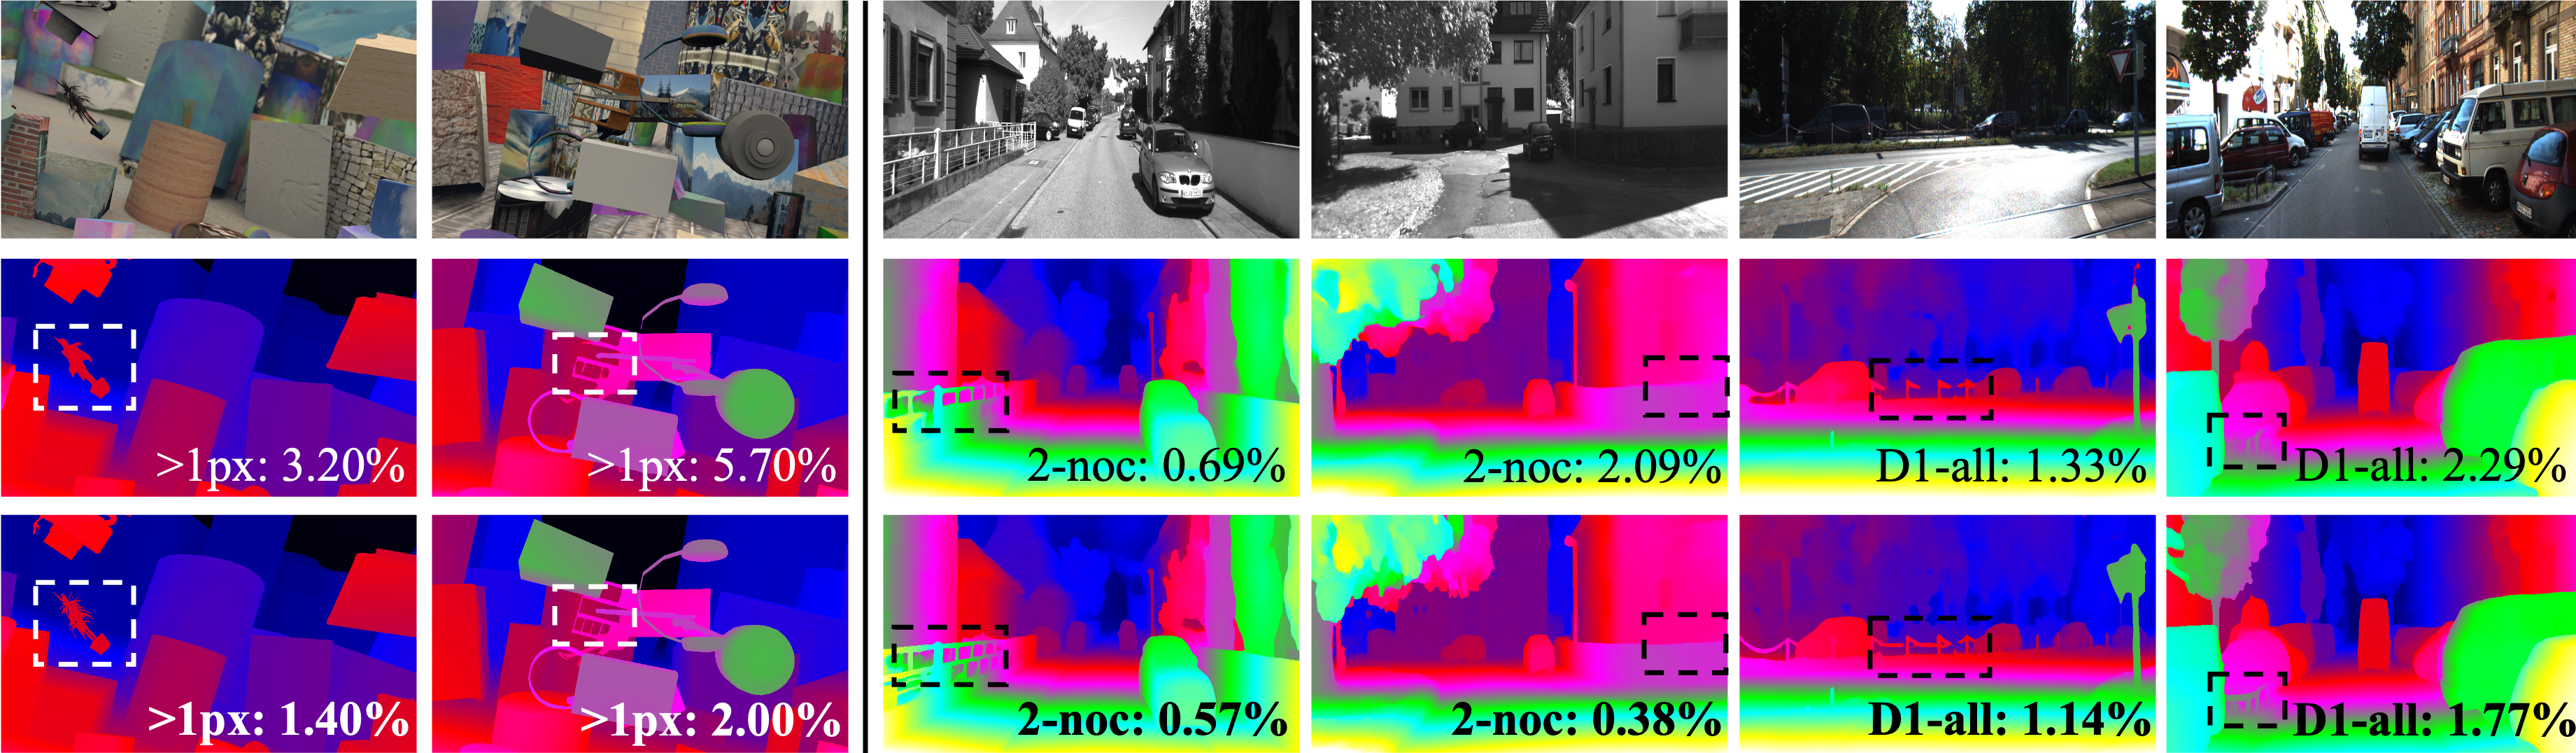
\includegraphics[width=0.97\linewidth]{fig/nmrf/sceneflow_kt.png}\\
	\end{tabular}
	\vspace{-0.8em}
	\caption{\textbf{Qualitative evaluation on SceneFlow~\cite{mayer2016large}, KITTI 2012~\cite{geiger2012we}, and KITTI 2015~\cite{menze2015object}.} Examples are organized from left to right as SceneFlow, KITTI 2012, and KITTI 2015, with two columns shown for each benchmark. The proposed method yields more coherent disparity predictions than LEAStereo~\cite{cheng2020hierarchical}, particularly in low-texture surfaces and regions containing fine geometric details.}
	\label{fig:sceneflow_kt}
	\vspace{-1.0em}
\end{figure}

Qualitative examples are shown in Figure~\ref{fig:sceneflow_kt}.
The predicted disparity maps preserve fine structures while remaining robust in low-texture regions.
To further examine boundary quality, we visualize reconstructed point clouds and compare them with those produced by LEAStereo~\cite{cheng2020hierarchical} and IGEV-Stereo~\cite{xu2023iterative}.
As illustrated in Figure~\ref{fig:nmrf_sharp}, the proposed method produces sharper discontinuities and substantially reduces bleeding artifacts~\cite{tosi2021smd}, which are particularly harmful for downstream 3D reconstruction and robotic perception.

\begin{figure}[!t]
	\centering
	\begin{subfigure}[t]{0.44\linewidth}
		\centering
		\tabcolsep=0.01cm
		\renewcommand*{\arraystretch}{0.35}
		\begin{tabular}{c c}
			\raisebox{0.0em}{\rotatebox{90}{\scriptsize \textsf{LEAStereo~\cite{cheng2020hierarchical}}}} 
			& 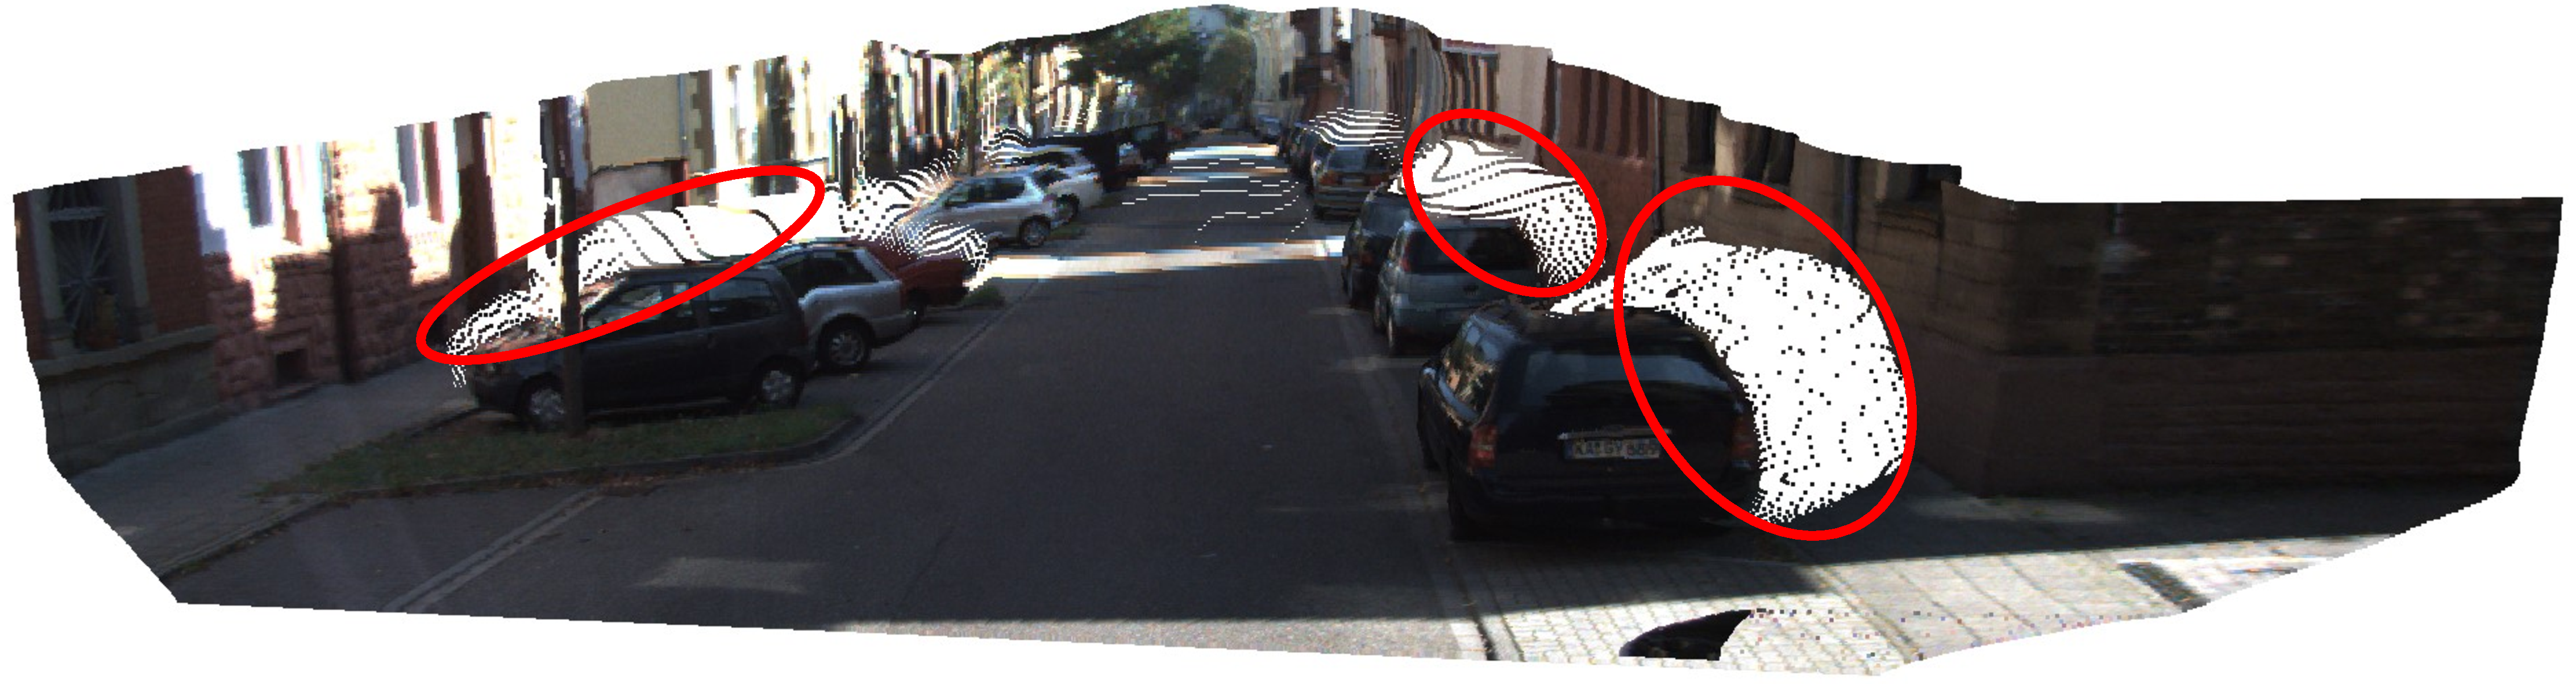
\includegraphics[width=0.88\linewidth]{fig/nmrf/leastereo.pdf} \\
			
			\raisebox{0.5em}{\rotatebox{90}{\scriptsize \textsf{IGEV~\cite{xu2023iterative}}}} 
			& 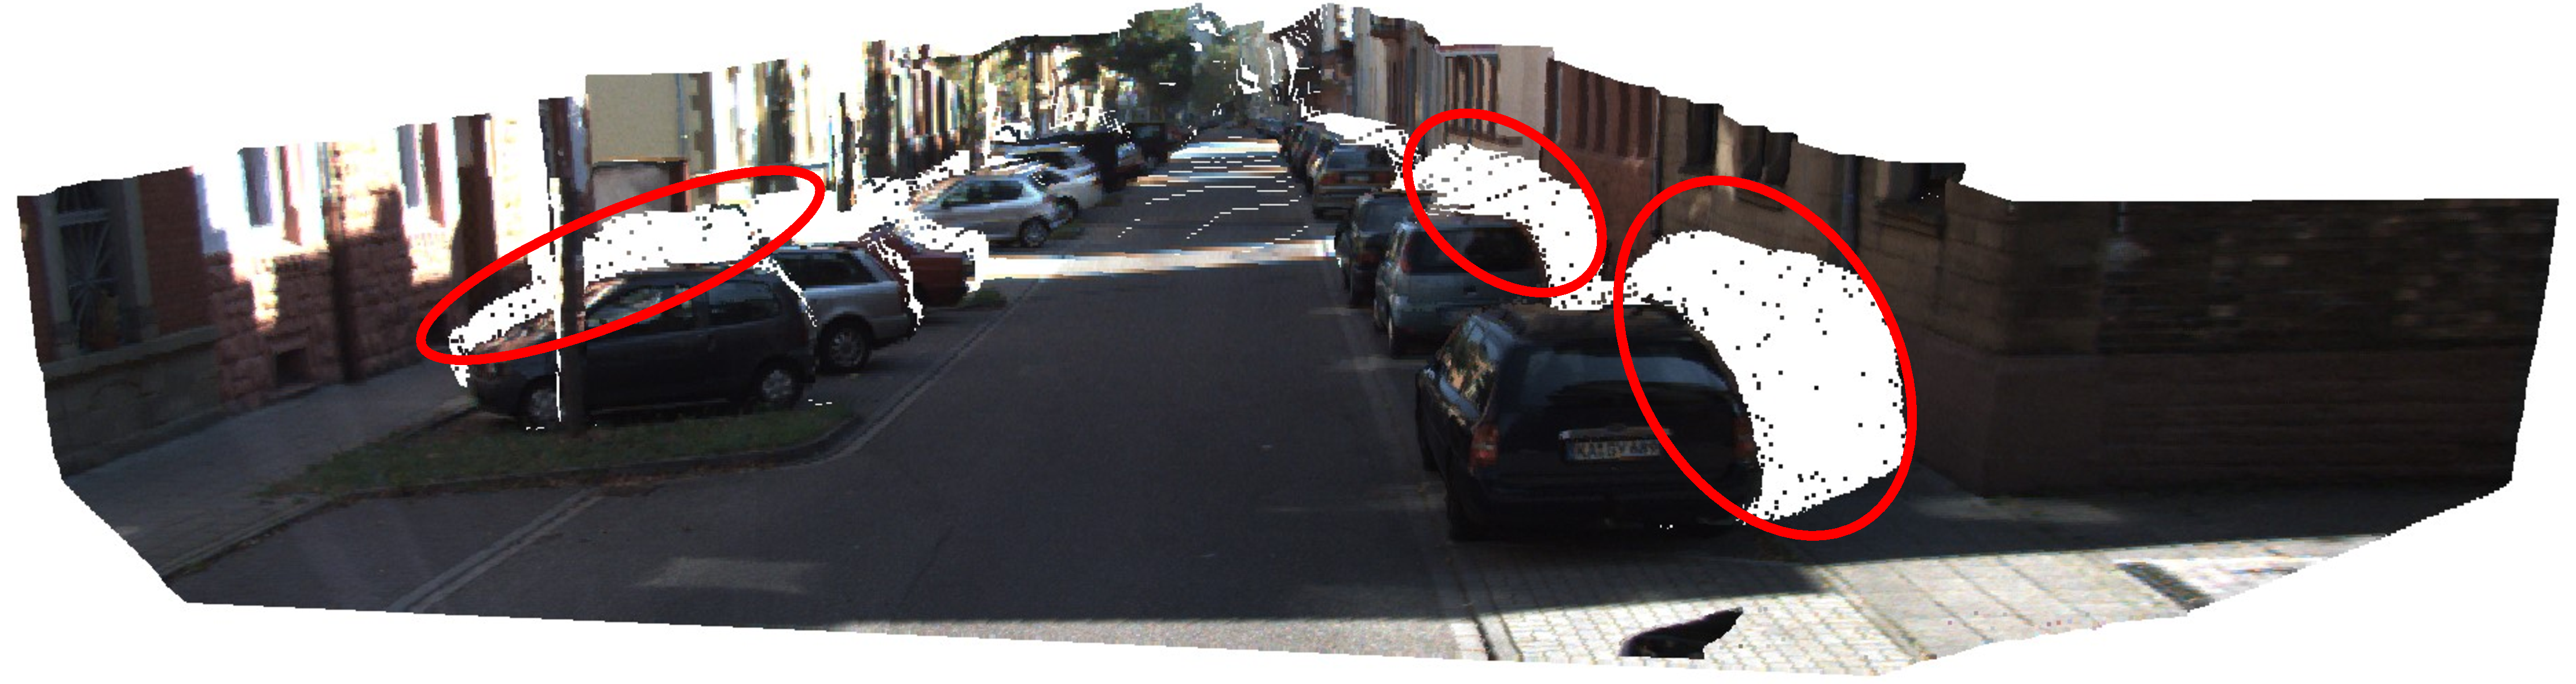
\includegraphics[width=0.88\linewidth]{fig/nmrf/igev.pdf} \\
			
			\raisebox{1.2em}{\rotatebox{90}{\scriptsize \textsf{Ours}}} 
			& 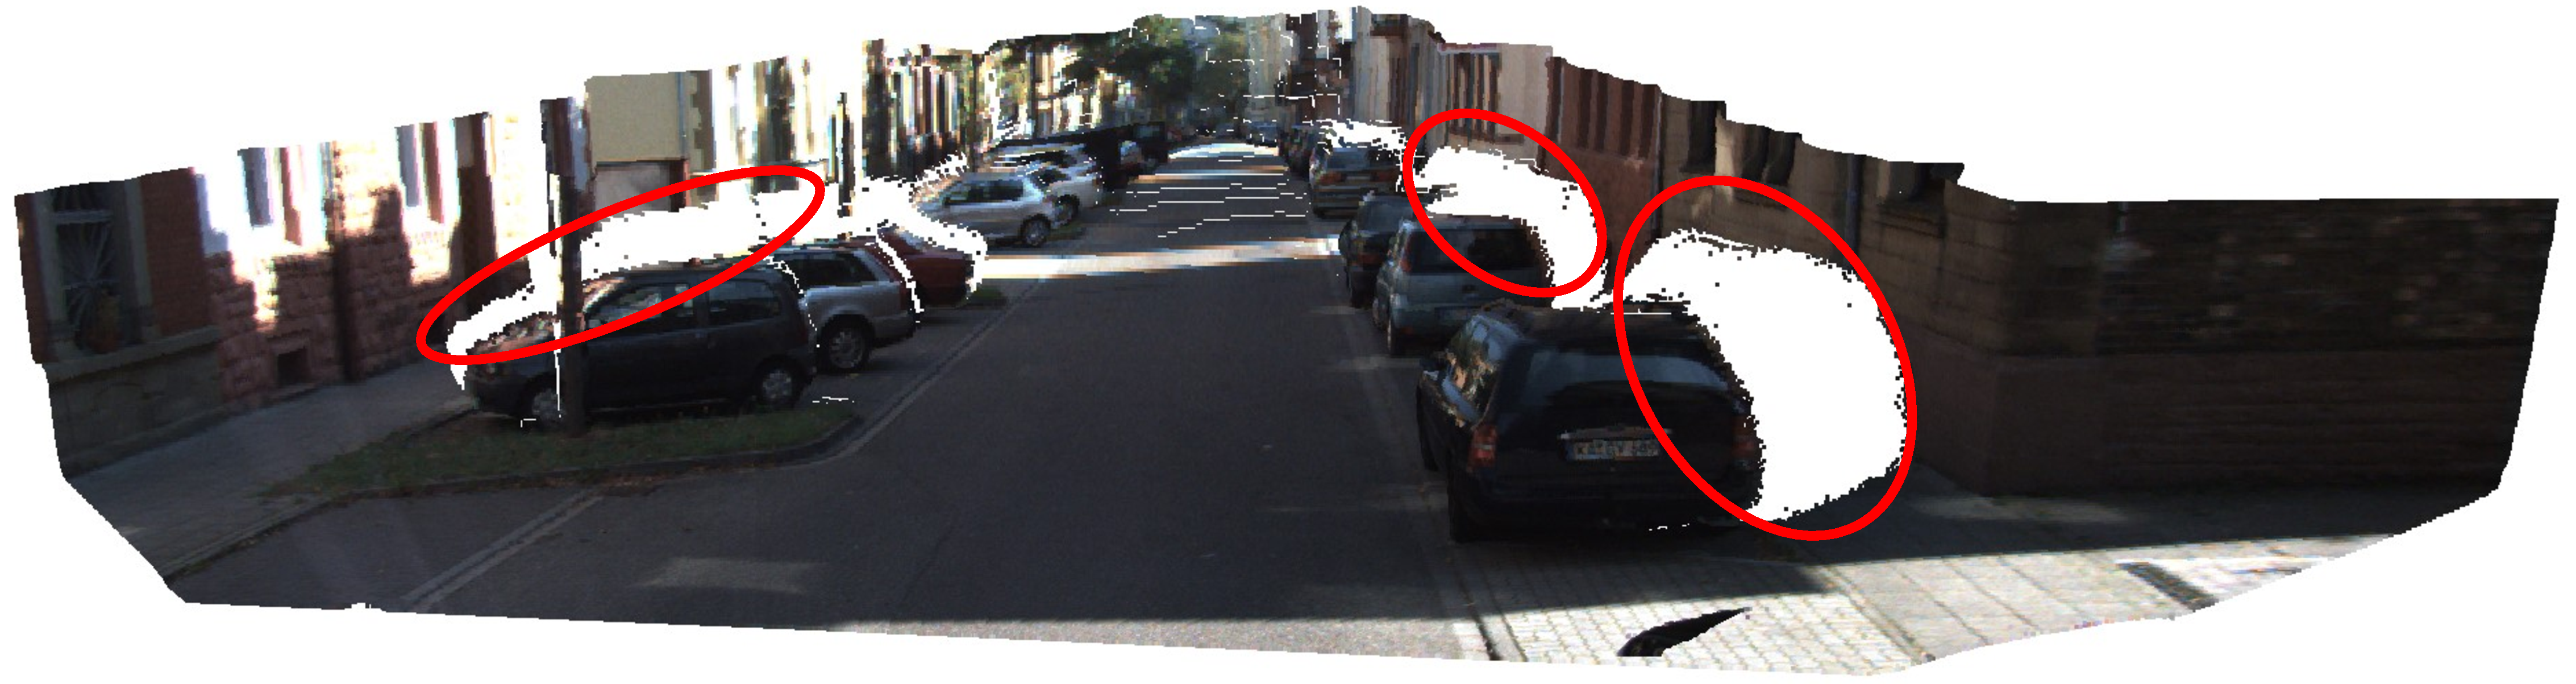
\includegraphics[width=0.88\linewidth]{fig/nmrf/nmrf.pdf}
		\end{tabular}
		\vspace{-0.2em}
		\caption{\small KITTI point-cloud reconstruction}
		\label{fig:nmrf_sharp}
	\end{subfigure}
	\hfill
	\begin{subfigure}[t]{0.55\linewidth}
		\centering
		\tabcolsep=0.01cm
		\renewcommand*{\arraystretch}{0.35}
		\begin{tabular}{c c}
			\raisebox{1.8em}{\rotatebox{90}{\scriptsize \textsf{Middlebury}}} 
			& 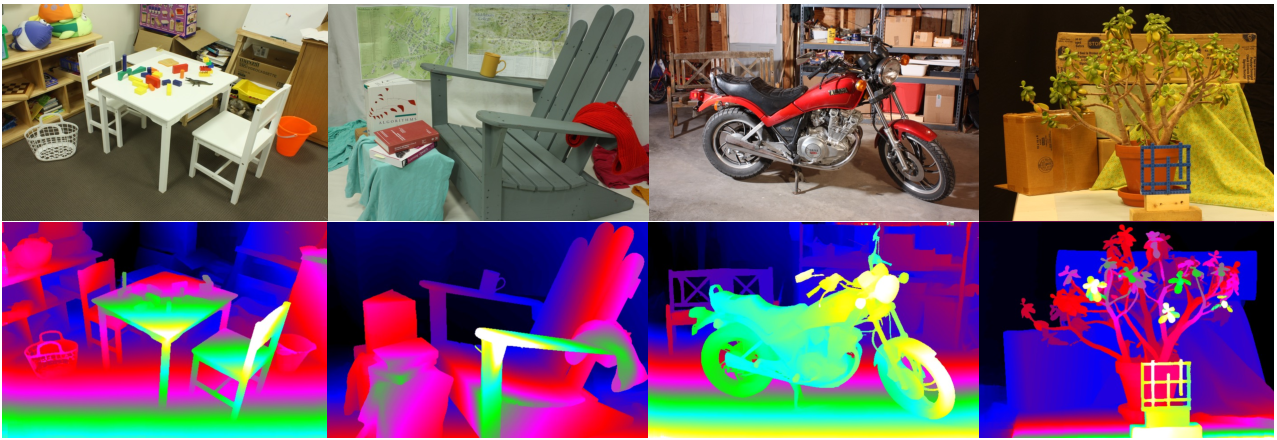
\includegraphics[width=0.88\linewidth]{fig/nmrf/middlebury.pdf} \\
			
			\raisebox{1.9em}{\rotatebox{90}{\scriptsize \textsf{ETH3D}}} 
			& 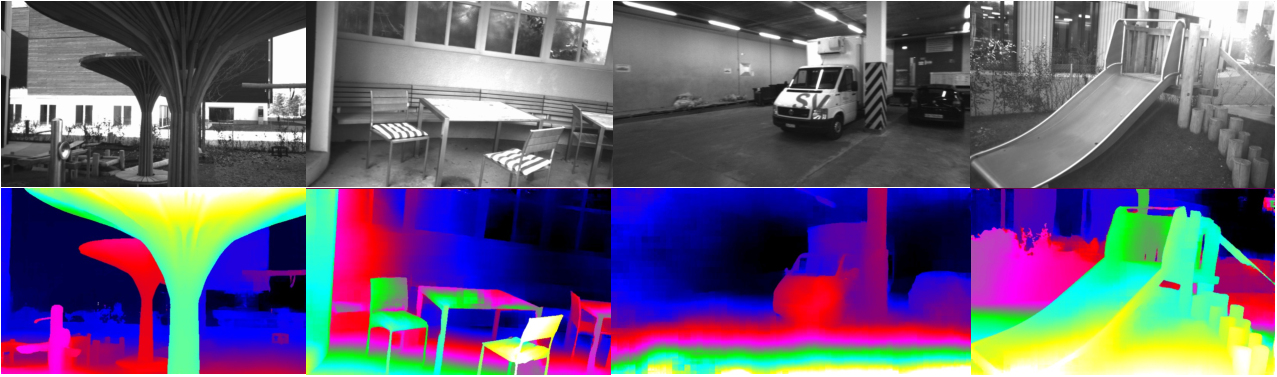
\includegraphics[width=0.88\linewidth]{fig/nmrf/eth3d.pdf}
		\end{tabular}
		
		\vspace{0.1em}
		\caption{\small Zero-shot generalization}
		\label{fig:qua-zero_shot}
	\end{subfigure}
	\vspace{-1.0em}
	\caption{\textbf{Qualitative evaluation of reconstruction quality and cross-dataset generalization.}
	(a) Point-cloud reconstruction results on the KITTI test set. Compared with LEAStereo~\cite{cheng2020hierarchical} and IGEV~\cite{xu2023iterative}, the proposed NMRF method produces sharper geometric boundaries and reduces bleeding artifacts around object contours.
	(b) Zero-shot qualitative results on Middlebury and ETH3D, demonstrating the generalization ability of the proposed method across datasets with different scene structures and imaging conditions.}
	\vspace{-0.5em}
\end{figure}

\subsection{Zero-Shot Generalization}

A stereo model trained on synthetic data should transfer reliably to real-world domains, since acquiring dense and accurate real-world disparity annotations is expensive and often impractical.
To assess this ability, we train models only on SceneFlow and directly evaluate them on KITTI, Middlebury, and ETH3D without any target-domain fine-tuning.
The quantitative results are reported in Table~\ref{tab:results_zero_shot}.
The proposed method demonstrates strong cross-domain robustness and outperforms DSMNet~\cite{zhang2020domain} and CREStereo++~\cite{jing2023uncertainty}, both of which are specifically designed to improve domain generalization.
This result indicates that the proposed candidate-label representation and neural MRF inference can capture transferable geometric structure rather than overfitting to synthetic appearance statistics.
The real-time \emph{NMRF-light} variant remains competitive, although its generalization performance is slightly lower than that of the original NMRF configuration.
Qualitative zero-shot results on ETH3D and Middlebury are provided in Figure~\ref{fig:qua-zero_shot}, showing that the model generalizes to diverse image conditions, including indoor scenes, grayscale images, and high-resolution stereo pairs.


\subsection{Ablation Studies}
We conduct ablation studies to analyze the contribution of the main architectural components.
For efficiency, all ablation experiments use the lightweight ResNet backbone unless otherwise specified.

\noindent\textbf{Effectiveness of the Disparity Proposal Network.} The quality of candidate labels is critical because the subsequent neural MRF inference is performed over the proposed hypothesis set.
If the correct disparity is not covered by any candidate, later message passing cannot fully recover it.
We therefore evaluate the Disparity Proposal Network (DPN) using two metrics.
The first is $x$-pixel recall, defined as the percentage of pixels for which at least one candidate label lies within $x$ pixels of the ground-truth disparity.
The second is the EPE between the ground-truth disparity and the closest candidate label.
As shown in Table~\ref{tab:proposal_quality}, the DPN significantly improves the quality of candidate hypotheses compared with the initialized label seeds.
At the 8-pixel threshold, corresponding to one pixel at the coarse feature resolution, the generated candidates achieve 99.8\% recall across commonly used datasets.
Moreover, the candidate-label EPE is substantially lower than the final disparity EPE, for example 0.22 versus 0.45 on SceneFlow.
These results demonstrate that the DPN provides a highly reliable hypothesis set and is unlikely to be the bottleneck of the overall framework.

\begin{table}[!t]
	\small
	\centering
	\caption{
	\textbf{Zero-shot generalization and ablation studies.}
	(a) zero-shot evaluation across KITTI 2012, KITTI 2015, Middlebury, and ETH3D. (b) ablation study on the SceneFlow test set.
	}
	\vspace{-1.0em}
	\begin{subtable}[t]{0.58\linewidth}
		\centering
		\scriptsize
		%\renewcommand{\arraystretch}{1.05}
		%\setlength{\tabcolsep}{1.8pt}
		\caption{\footnotesize Zero-shot generalization}
		\label{tab:results_zero_shot}
		\begin{tabular}{l c c c c}
			\toprule
			Method 
			& KITTI-12 
			& KITTI-15 
			& Midd. $\nicefrac{1}{4}$ 
			& ETH3D \\
			\midrule
			DSMNet~\cite{zhang2020domain} 
			& 6.2 & 6.5 & 8.1 & 6.2 \\
			RAFT-Stereo~\cite{lipson2021raft} 
			& 4.7 & 5.5 & 9.4 & \textbf{3.3} \\
			CREStereo++~\cite{jing2023uncertainty} 
			& 4.7 & \underline{5.2} & -- & 4.4 \\
			IGEV-Stereo~\cite{xu2023iterative} 
			& 5.2 & 5.7 & 8.8 & 4.0 \\
			\midrule
			NMRF 
			& \textbf{4.2} & \textbf{5.1} & \textbf{7.5} & 3.8 \\
			NMRF-light 
			& \underline{4.5} & 5.3 & \underline{8.0} & \underline{3.7} \\
			\bottomrule
		\end{tabular}
	\end{subtable}
	\hfill
	\begin{subtable}[t]{0.39\linewidth}
		\centering
		\scriptsize
		%\renewcommand{\arraystretch}{1.05}
		%\setlength{\tabcolsep}{2.0pt}
		\vspace{-0.5em}
		\caption{\footnotesize Component ablation}
		\label{tab:ablation_comp}
		\begin{tabular}{l c c c}
			\toprule
			Variant 
			& EPE 
			& Bad1.0 
			& Time \\
			\midrule
			baseline 
			& 0.58 & 5.96 & 0.064 \\
			w/ adaptive bias 
			& 0.57 & 5.80 & 0.067 \\
			w/ position aggregation 
			& 0.57 & 5.53 & 0.072 \\
			w/ \textit{shared} self edges 
			& 0.56 & 5.48 & 0.072 \\
			w/ self edges 
			& 0.53 & 5.24 & 0.081 \\
			\rowcolor{lightgray}
			w/ refinement 
			& 0.45 & 4.50 & 0.101 \\
			w/ refinement $\times 2$ 
			& 0.43 & 4.13 & 0.121 \\
			\bottomrule
		\end{tabular}
	\end{subtable}
\end{table}

\noindent\textbf{Number of candidate labels.} The number of candidate labels controls the trade-off between hypothesis diversity, computational cost, and inference stability.
In the main experiments, \emph{NMRF-light} uses two candidate labels per pixel, while \emph{NMRF-SwinT} uses four.
We further vary the number of labels $K$ to study its influence on accuracy, generalization, and runtime.
As shown in Figure~\ref{fig:k_boxplot}a, the model remains competitive even with a single candidate label, indicating that the proposal network often produces highly accurate hypotheses.
Increasing $K$ can improve candidate diversity, but the gain is not strictly monotonic.
When too many candidates are retained, inaccurate hypotheses may also enter the MRF inference stage and increase ambiguity.
For example, using six candidates does not consistently outperform using five.
Overall, $K=2$ offers a favorable accuracy-efficiency balance and is therefore adopted in the real-time model.

\begin{figure}[!t]
	\centering
	\vspace{1.5em}
	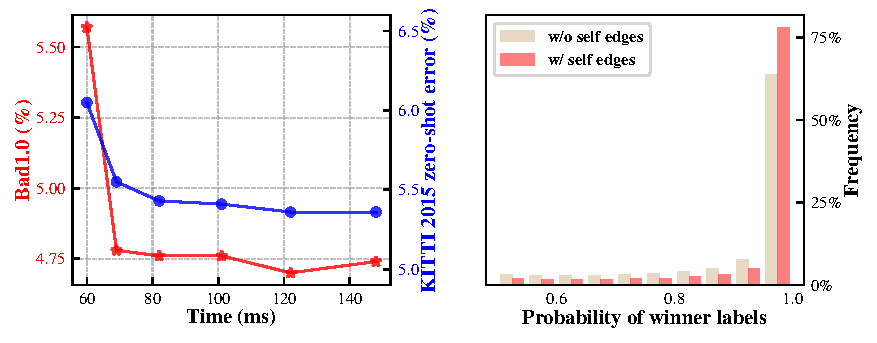
\includegraphics[width=0.96\linewidth]{fig/nmrf/ablation.pdf}\\
	\vspace{-0.2em}
	\makebox[0.5\linewidth]{\hspace{1em}\footnotesize (a)}
	\makebox[0.02\linewidth]{}
	\makebox[0.45\linewidth]{\hspace{-1em}\footnotesize (b)}\\
	\vspace{-0.5em}
	\caption{
		\textbf{Effect of candidate-label cardinality and self-edge propagation.}
		(a) Comparison of accuracy, inference time, and zero-shot generalization as the number of candidate labels varies from 1 to 6.
		(b) Histogram of the posterior probability associated with the winning label. Self-edge message passing makes the inferred label distributions more peaked, assigning higher probability to the selected candidate. The statistics are collected from 4.5M uniformly sampled pixels on the SceneFlow test set.
	}
	\label{fig:k_boxplot}
	\vspace{-1.0em}
\end{figure}

\noindent\textbf{Role of self edges.} We next study the role of self edges in neural MRF inference.
Unlike conventional stereo MRF formulations, where message passing is mainly defined between neighboring pixels, our model also allows information exchange among candidate labels belonging to the same pixel.
This design enables the network to reason about intra-pixel competition and reinforce the most plausible hypothesis.
As shown in Table~\ref{tab:ablation_comp}, including self edges improves disparity accuracy, reducing EPE from 0.57 to 0.53.
Figure~\ref{fig:k_boxplot}b depicts that self-edge message passing helps sharpen the posterior distribution over candidate labels and allows the loss in Equation~\ref{eq:loss-est} to more effectively emphasizing the selected hypothesis.
We also compare against a variant that shares the same potential function for self and neighboring edges ($4^{\mathrm{th}}$ row in Table~\ref{tab:ablation_comp}).
The performance drop of this shared-potential variant confirms that intra-pixel and spatial interactions should be modeled with distinct functions.

\noindent\textbf{Attentional aggregation components.} We further evaluate the two attentional aggregation designs in Equation~\ref{eq:nmrf_agg}: content-adaptive positional bias and position aggregation.
The results in Table~\ref{tab:ablation_comp} show that both components reduce disparity estimation outliers.
The content-adaptive positional bias is particularly beneficial around object boundaries, where aggregation should be sensitive to local appearance structure.
This behavior is consistent with the sharp discontinuities observed in Figure~\ref{fig:nmrf_sharp}.
Position aggregation, which injects positional information into the value branch, contributes more strongly to overall accuracy and improves predictions in broad textureless regions, as illustrated in Figure~\ref{fig:sceneflow_kt}.
Together, these two components make message aggregation both geometry-aware and content-adaptive.

\noindent\textbf{Disparity refinement.} Finally, we analyze the effect of the refinement module.
Among the components listed in Table~\ref{tab:ablation_comp}, the refinement module brings the largest performance gain.
This is expected because fine-level features at $\nicefrac{1}{4}$ resolution contain spatial details that are not fully preserved during coarse-level proposal extraction and MRF inference.
The refinement module therefore plays an important role in recovering thin structures, sharpening boundaries, and improving local disparity coherence.
Adding a second refinement module further improves in-domain accuracy but slightly weakens cross-domain generalization, as shown the last row of Table~\ref{tab:ablation_comp}.
This trade-off suggests that additional refinement can better fit the training distribution, while a simpler refinement design may preserve better robustness under domain shift.
In practice, the number of refinement stages can be chosen according to the target application, depending on whether maximum benchmark accuracy or stronger generalization is preferred.

\begin{table}[!t]
	\small
	\centering
	\caption{
		\textbf{Analysis of disparity proposal quality and seed propagation design.}
		(a) We evaluate the quality of the proposed disparity candidates on SceneFlow and KITTI validation splits. (b) We compare two attention patterns used for propagating label seeds. Candidate recall is measured by the percentage of pixels whose candidate set contains a label within a given threshold, while final disparity quality is measured by EPE and Bad 1.0.
	}
	\vspace{-0.5em}
	\begin{subtable}[t]{0.52\linewidth}
		\centering
		\scriptsize
		\caption{Quality of generated disparity candidates.
		}
		\label{tab:proposal_quality}
		\setlength{\tabcolsep}{2.2pt}
		\renewcommand{\arraystretch}{1.05}
		\begin{tabular}{c c c c c c}
			\toprule
			& \multicolumn{3}{c}{candidate labels} & \multicolumn{2}{c}{label seeds}\\
			\cmidrule(lr){2-4}
			\cmidrule(lr){5-6}
			Datasets & 3px & 8px & EPE & 8px & 16px \\
			& [\%]$\uparrow$ & [\%]$\uparrow$ & [px]$\downarrow$ & [\%]$\uparrow$ & [\%]$\uparrow$\\
			\cmidrule(lr){1-4}
			\cmidrule(lr){5-6}
			SceneFlow-test & 99.29 & 99.77 & 0.22 & 91.94 & 94.85\\
			KITTI-12 \textit{val} & 98.88 & 99.72 & 0.31 & 93.87 & 95.89\\
			KITTI-15 \textit{val} & 99.66 & 99.95 & 0.21 & 93.91 & 95.92\\
			\bottomrule
		\end{tabular}
	\end{subtable}
	\hfill
	\begin{subtable}[t]{0.44\linewidth}
		\centering
		\scriptsize
		\caption{Effect of the attention pattern for seed propagation.}
		\label{tab:proposal_attention}
		\setlength{\tabcolsep}{2.4pt}
		\renewcommand{\arraystretch}{1.05}
		\begin{tabular}{c c c c c c}
			\toprule
			& \multicolumn{2}{c}{candidate labels} & \multicolumn{2}{c}{disparity estimation}\\
			\cmidrule(lr){2-3}
			\cmidrule(lr){4-5}
			& 3px & 8px  & EPE & Bad 1.0 \\
			& [\%]$\uparrow$ & [\%]$\uparrow$ & [px]$\downarrow$ & [\%]$\downarrow$ \\
			\cmidrule(lr){1-3}
			\cmidrule(lr){4-5}
			cross-shaped & 99.29 & 99.77  & 0.45 & 4.50\\
			local window & 99.18 & 99.72 & 0.47 & 4.56 \\
			\bottomrule
		\end{tabular}
		
	\end{subtable}
	
	%\vspace{-0.5em}
	\label{tab:res_proposal}
	%\vspace{-1.7em}
\end{table}

\section{Application in Road Surface Perception}
The geometric profile of road surfaces critically impacts the driving performance of autonomous vehicles, as surface irregularities, such as bumps, potholes, and subtle elevation changes, can compromise vehicle stability, traction, and control.
Accurate, real-time perception of these features is essential for adaptive path planning, suspension control, and collision avoidance.
However, conventional sensing modalities face significant limitations in meeting the dual requirements of dense metric accuracy and operational robustness.
While LiDAR provides precise 3D measurements, its sparse point density (typically $< 100\,\mathrm{pt/m}^2$ at a $10\,\mathrm{m}$ range) limits its ability to capture fine-grained road elevation variations, such as cracks or shallow potholes with depths under $5\,\mathrm{cm}$.
Moreover, the high sensor cost and mechanical complexity of LiDAR hinder its widespread deployment in cost-sensitive applications.
Monocular depth estimation, although more cost-effective and lower in maintenance, faces challenges such as inherent scale ambiguity and instability in texture-scarce regions.
These issues are common to homogeneous paved roads, where elevation changes often lack distinct visual cues. Stereo vision addresses these gaps by providing dense, metric depth estimation at moderate cost, making it uniquely suited for detecting subtle road surface irregularities.
However, a critical challenge arises in this application: road surfaces often exhibit large textureless regions (\eg, uniform asphalt or concrete), where conventional stereo matching algorithms struggle due to insufficient intensity variations for reliable correspondence estimation.
Our NMRF architecture overcomes this limitation through long-range, data-dependent message passing, which propagates disparity hypotheses from geometrically confident regions (\eg, textured edges, lane markings) into textureless areas. 
Learned attention rules dynamically prioritize message from reliable neighbors, enabling the model to infer disparities via global structural reasoning rather than error-prone local matching.
For example, in flat road segments, the system synthesizes depth estimates by extrapolating cues from adjacent lane markings (top row of Figure~\ref{fig:road-ele}), effectively ``hallucinating'' plausible geometry where texture is absent.

To evaluate our architecture's road surface perception capability, we utilize the Road Surface Reconstruction Dataset (RSRD)~\cite{zhao2024road}, a specialized benchmark for road geometry analysis. 
RSRD contains 2,800 high-resolution stereo pairs ($1920 \times 1080$) with centimeter-level elevation ground truth derived from LiDAR-acquired disparities and 6-DoF poses.
The dataset focuses on diverse asphalt/concrete road conditions, including potholes, speed bumps, cracks, and subtle depressions, under varying illumination.
For texture-scarce evaluation, we adopt RoadBEV's~\cite{zhao2024roadbev} 1,210/371 train-test split at $960 \times 540$ resolution, prioritizing sequences with severe unevenness and minimal road markings. 
This configuration mirrors real-world challenges where homogeneous regions dominate and local textures are inadequate for conventional stereo matching. RSRD's sparse-texture, high-precision design provides a rigorous testbed for safety-critical automotive depth estimation systems.
For fair comparison, the evaluation region of interest (RoI) in Figure~\ref{fig:road-ele} aligns with the benchmark's prior work~\cite{zhao2024roadbev}, covering lateral and longitudinal ranges of $[-1.0\mathrm{m},0.9\mathrm{m}]$ and $[2.1\mathrm{m},7.1\mathrm{m}]$, respectively.
\begin{figure}[!t]
	\centering
	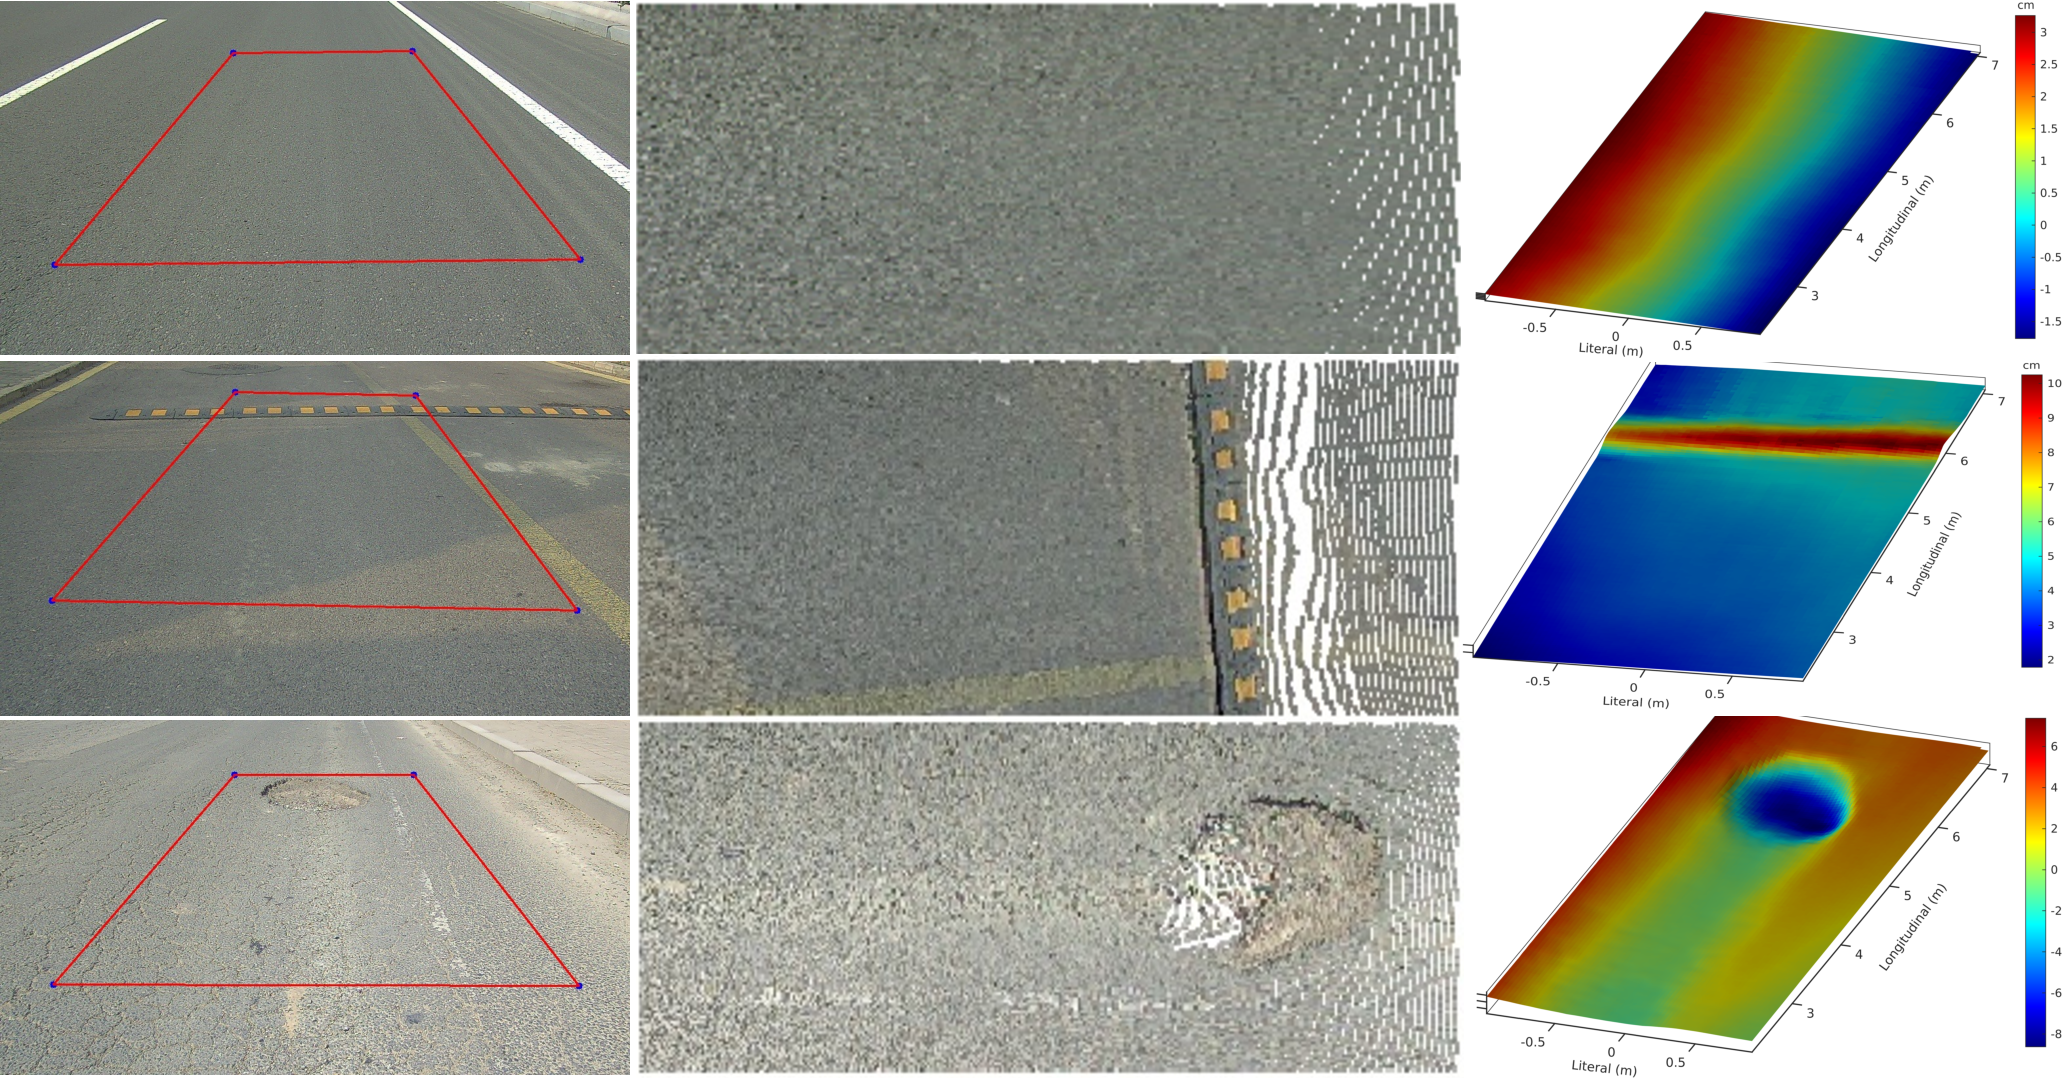
\includegraphics[width=0.99\linewidth]{fig/nmrf/elevation.pdf}
	%\vspace{-0.3em}
	\caption{\textbf{Visualization of road surface reconstruction using our method.} From left to right: left images, recovered road point clouds in a bird's-eye view, and estimated road meshes with colored elevation. Only the road surface within the region of interest (ROI) is visualized and evaluated.}
	\label{fig:road-ele}
\end{figure}

\section{Conclusion}
This chapter presented a neural Markov random field architecture for stereo matching.
Instead of relying on dense cost volume aggregation or recurrent ConvGRU refinement, the proposed method formulates stereo disparity estimation as structured inference over a compact set of candidate disparity labels.
This design retains the structural bias of classic MRF-based stereo methods while allowing the inference process to be learned end-to-end.
Experiments on synthetic and real-world benchmarks demonstrated strong accuracy, robust cross-domain generalization, and competitive efficiency. 
Within this thesis, this chapter establishes the stereo correspondence foundation for learning visual geometry, which will be extended in later chapters by incorporating additional sources of depth and motion cues.